\documentclass[12pt]{article}

% -----------------------------------------------------------------------------
% Page size, margins, font encoding, and base fonts
% -----------------------------------------------------------------------------
\usepackage[margin=1in]{geometry}
\usepackage[T1]{fontenc}
\usepackage[utf8]{inputenc}
\usepackage{textcomp}
\usepackage{newtxtext,newtxmath}

% -----------------------------------------------------------------------------
% Core packages
% -----------------------------------------------------------------------------
\usepackage{amsmath}
\usepackage{graphicx}
\usepackage{booktabs}
\usepackage{array}
\usepackage{longtable}
\usepackage{calc}
\usepackage{float}
\usepackage{caption}
\usepackage{setspace}
\usepackage{lineno}
\usepackage{xcolor}
\usepackage[round,authoryear]{natbib}
\usepackage{hyperref}
\usepackage{bookmark}
\IfFileExists{xurl.sty}{\usepackage{xurl}}{}
\urlstyle{same}

% -----------------------------------------------------------------------------
% Review-manuscript layout for Computers and Electronics in Agriculture:
% single column, 12 pt, 1 inch margins, double-spaced main text.
% -----------------------------------------------------------------------------
\pagestyle{plain}
\doublespacing
\setlength{\parindent}{0pt}
\setlength{\parskip}{0pt}
\setlength{\emergencystretch}{3em}

% -----------------------------------------------------------------------------
% Section heading format
% -----------------------------------------------------------------------------
\usepackage{titlesec}
\titleformat{\section}
  {\normalfont\large\bfseries}
  {\thesection}{0.75em}{}
\titleformat{\subsection}
  {\normalfont\normalsize\bfseries}
  {\thesubsection}{0.75em}{}
\titleformat{\subsubsection}
  {\normalfont\normalsize\itshape}
  {\thesubsubsection}{0.75em}{}
\titlespacing*{\section}{0pt}{1.2em}{0.6em}
\titlespacing*{\subsection}{0pt}{1.0em}{0.45em}
\titlespacing*{\subsubsection}{0pt}{0.8em}{0.35em}

% -----------------------------------------------------------------------------
% Caption and table font standards
% -----------------------------------------------------------------------------
\newcommand{\tablecaptionfontsize}{\fontsize{10pt}{12pt}\selectfont}
\newcommand{\tablefontsize}{\fontsize{9pt}{11pt}\selectfont}
\DeclareCaptionFont{captionten}{\fontsize{10pt}{12pt}\selectfont}
\captionsetup{
  font=captionten,
  labelfont=bf,
  textfont=captionten,
  justification=raggedright,
  labelsep=period,
  singlelinecheck=false
}
\newcolumntype{L}[1]{>{\tablefontsize\raggedright\arraybackslash}m{#1}}

% -----------------------------------------------------------------------------
% Hyperlink and bibliography helper commands
% -----------------------------------------------------------------------------
\providecommand{\tightlist}{\setlength{\itemsep}{0pt}\setlength{\parskip}{0pt}}
\providecommand{\DOIprefix}{doi: }
\providecommand{\URLprefix}{URL: }
\providecommand{\ArXivprefix}{arXiv: }
\providecommand{\Pubmedprefix}{PMID: }
\providecommand{\doi}[1]{\href{https://doi.org/\detokenize{#1}}{\nolinkurl{#1}}}
\hypersetup{
  pdftitle={GrapeMaster: A Crop-Season-Centered Digital Platform for Traceable Vineyard Disease Management},
  hidelinks,
  pdfcreator={LaTeX}
}

\newcommand{\figref}[1]{\hyperref[#1]{Figure~\ref*{#1}}}
\newcommand{\figpanelref}[2]{\hyperref[#1]{Figure~\ref*{#1}#2}}
\newcommand{\tabref}[2]{\hyperref[#1]{Table~#2}}

% -----------------------------------------------------------------------------
% Manuscript title
% -----------------------------------------------------------------------------
\newcommand{\manuscripttitle}{GrapeMaster: A Crop-Season-Centered Digital Platform for Traceable Vineyard Disease Management}

\begin{document}

\linenumbers

\begin{center}
{\LARGE\setstretch{0.9}\selectfont \manuscripttitle\par}
\end{center}

\vspace{0.8em}

\begingroup
\normalsize
\setstretch{1.05}
\noindent
\mbox{Author~information~to~be~completed~before~submission}
\par
\vspace{0.7em}

\noindent
Affiliations, author order, and corresponding author details will be completed before journal submission.
\par
\endgroup

\vspace{1em}

\section*{Abstract}

Grapevine is a high-value fruit crop. In humid subtropical vineyards, epidemic diseases, particularly downy mildew, are major constraints on yield, fruit quality, production cost, and sustainable management. Although disease warning, phenology simulation, image diagnosis, advisory support, and management records have each advanced, their outputs are still often handled as separate functions rather than as a shared seasonal management process. This creates a platform gap between analytical outputs and field action, treatment records, evidence retention, and season-level review. We developed GrapeMaster, a vineyard-level digital platform that uses the crop season as a shared management unit to organize analytical outputs and advisory interactions into executable and reviewable management actions. Backend verification showed that 126 crop seasons retained linked weather, phenology, disease-risk, model input-output, notification, task, fungicide-feedback, advisory, and message records, including feedback records used for protection-state updating. A representative season replay reconstructed the prediction--notification--task--treatment--review chain, showing that the platform can maintain continuity from risk interpretation to season-level review. Module-level validation further supported the analytical readiness of downy mildew warning, broad-stage phenology display, and grape disease image recognition for the Guangxi context. These results indicate that GrapeMaster offers a deployable platform architecture for converting isolated digital tools into season-long, evidence-based vineyard disease management, with potential value for improving vineyard-level management consistency, standardization, and digital transformation.

\noindent\textbf{Keywords:} grapevine; downy mildew; decision support system; crop-season management; digital agriculture; advisory support; record traceability

\section{Introduction}\label{introduction}

Grapevine is an important economic crop for fresh consumption, wine production, and processing. In humid subtropical vineyards, high humidity, rainfall, dew formation, and heterogeneous field microclimates readily favor epidemic diseases represented by downy mildew \citep{gesslerPlasmoparaViticolaReview2011,yuEffectsRainShelter2017,yuComparisonThreeTypes2022,pengAdvancesUnderstandingGrapevine2024}. In severe cases, this disease can cause more than 75\% yield loss in warm and humid grape-growing regions \citep{koledenkovaPlasmoparaViticolaCausal2022,pengAdvancesUnderstandingGrapevine2024}. However, conventional plant-protection practice often depends on fragmented field scouting, empirical spray calendars, manual symptom diagnosis, informal advisory sources with uneven documentation and reliability, and retrospective paper records. This non-integrative decision approach can lead to mismatches between spray timing and disease-risk periods, inappropriate pesticide concentration or mixing, and control outcomes that are difficult to trace and quantitatively evaluate \citep{pertotCriticalReviewPlant2017,rossiAddressingImplementationProblem2014,oliverFungicideUsePatterns2023,wiseSprayerTypeWater2010}.

Several analytical technologies relevant to vineyard disease management have advanced substantially. Grapevine downy mildew models have progressed from empirical warning rules to mechanistic or semi-mechanistic descriptions of pathogen development and infection processes \citep{orlandiniPLASMOSimulationModel1993,parkDMCASTPredictionModel1997,caffiMechanisticModelSimulating2011}, and warning systems can improve treatment timing when meteorological inputs, local calibration, and implementation context are adequate \citep{caffiEvaluationWarningSystem2010,caffiFungicideModelsAre2018,carisseDevelopmentGrapeDowny2016}. Grapevine phenology models provide crop-stage information for interpreting host susceptibility, warning windows, canopy development, and operation timing \citep{caffarraIncreasingRobustnessPhenological2010,parkerGeneralPhenologicalModel2011,garciadecortazar-atauriGrapevinePhenologyFrance2017,wangAssessingGrapevinePhenological2020}. Image-recognition and advisory systems can convert visible symptoms into structured diagnostic evidence and management-oriented explanation \citep{yanAFMYOLOv8sAccurateFast2024,yanCDIPChatGLM3DualmodelApproach2025,shafayEndtoendVisionLanguage2026,raiAdvancingSitespecificDisease2026}. These technologies are valuable in their respective roles; the challenge for extension and industrial deployment is how to coordinate their separate outputs within a shared seasonal management context.

More broadly, digital agriculture and DSS implementation studies increasingly show that production deployment is not determined by model performance alone. Operational systems require stable data ingestion, modular architecture, reliable service operation, user-facing task processes, feedback mechanisms, record tracking, workflow evaluation, and traceability. End-to-end IoT and remote-sensing platforms demonstrate how heterogeneous data streams, analytics, and interfaces can be connected for complex agricultural management \citep{bakirScalableEndtoendIoT2026,nkwochaEndtoendDigitalFramework2025}. Public DSS and implementation studies further show that decision tools must be accessible, interpretable, and compatible with actual advisory and grower workflows \citep{seemForecastingPlantDisease2004,rossiAddressingImplementationProblem2014,bregaglioPublicDecisionSupport2022,rossiSharingDecisionmakingTools2023,gonzalez-dominguezPlantDiseaseModels2023}. These requirements shift attention from individual analytical functions to the platform architecture that can deliver, record, act upon, update, and review their outputs within a traceable workflow.

However, for grape production, the unresolved problem is not only whether individual models or diagnostic tools can perform well, but whether their outputs can be organized into a verifiable seasonal decision chain. Disease-risk models can identify infection windows and phenology models can describe crop-stage progression \citep{caffarraIncreasingRobustnessPhenological2010,puellesPredictiveModelsGrape2024}, while image-recognition and advisory tools can support symptom-level diagnosis and management-oriented explanation \citep{yanCDIPChatGLM3DualmodelApproach2025,shafayEndtoendVisionLanguage2026,raiAdvancingSitespecificDisease2026}. Yet these outputs often remain detached from the operational sequence of warning delivery, task generation, task completion, treatment feedback, later risk-state updating, symptom evidence, and season review. This creates a traceability gap: after a warning is generated, the system may not be able to reconstruct whether the warning was delivered, reviewed, converted into an operation, reflected in later protection status, and preserved as evidence for subsequent evaluation.

To address this gap, we developed and deployed GrapeMaster as a crop-season-centered, closed-loop, and traceable vineyard disease-management platform. In this architecture, the crop season is defined as the primary management unit for linking field identity, environmental state, crop development, disease-risk interpretation, warning delivery, task execution, treatment feedback, symptom evidence, advisory interaction, and archived records. The central research question was whether this platform-implemented architecture can convert separate analytical and operational functions into a verifiable workflow linking prediction, action, feedback, evidence, and review across the crop season. We evaluated this question through three evidence levels: the crop-season data model and database relationships that implement this management unit, workflow constraints and state-transition logic, and backend-record verification using linkage checks and representative season replay. By organizing analytical outputs, field operations, feedback records, and evidence review around the crop-season management unit, GrapeMaster provides a platform-level pathway for more consistent, standardized, traceable, and evaluable disease management in perennial fruit production.

\section{Materials and methods}\label{materials-and-methods}

\subsection{Study design, evidence sources, and vineyard context}\label{study-design-evidence-sources-and-vineyard-context}

\subsubsection{Study design and verification strategy}\label{study-design-and-verification-strategy}

This study describes the design, deployment, and record-based evaluation of GrapeMaster, a crop-season-centered digital platform for grapevine disease management. The platform workflow includes crop-season setup, weather and phenology updating, disease-risk warning, plant-protection task management, post-treatment protection-state updating, image-assisted disease diagnosis, LLM-assisted consultation, and management-record archiving.

The evaluation used two complementary evidence streams. Backend records from the deployed platform were used to evaluate whether mobile functions, backend services, database objects, scheduled workflows, notification and task services, image-upload pathways, advisory records, and crop-season records were linked as a functioning management workflow. Module-level validation evidence was used to characterize analytical components that can operate within this workflow.

The analytical layer includes a downy mildew initial-infection model for first seasonal infection-period warning, a phenology module for crop-stage interpretation, a grape-focused image-recognition module for symptom evidence, and an LLM advisory module for season-long consultation and management-oriented explanation. These modules were evaluated according to their platform roles and input--output compatibility with the crop-season workflow; additional module-level technical details are provided in Supplementary Table S2.

\subsubsection{Study area and field data sources}\label{study-area-and-field-data-sources}

The analytical modules were configured and evaluated for humid subtropical vineyard management using field data from Guangxi, China. This evidence base included meteorological records, grapevine phenological observations, airborne sporangia monitoring, symptom observations, and management records collected from field experiments and related vineyard observations. These regional data supported the FSIM-S downy mildew risk engine, phenology calibration, and grape disease image expansion used in the platform-compatible analytical configuration. Field and experimental data were analyzed separately from the backend operational records generated by the deployed GrapeMaster platform.

Consequently, module-level results are interpreted for the Guangxi humid subtropical vineyard configuration.

\subsection{Platform architecture and crop-season data model}\label{platform-architecture-and-crop-season-data-model}

\subsubsection{Software architecture and service layers}\label{software-architecture-and-service-layers}

GrapeMaster uses a layered architecture in which the mobile client, backend services, analytical model services, persistent storage, and external data sources are separated into logical service layers. The crop season is the central platform design unit linking a vineyard field with cultivar information, cultivation method, vine age, weather history, phenology outputs, disease-risk simulations, fungicide applications, plant-protection tasks, notes, image records, messages, and notifications. At the implementation level, the formal crop-season object, database relationship rules, workflow state-transition rules, and verification rules are specified in Supplementary Tables S4--S7.

Table~\ref{tab:architecture_layers} summarizes the five logical layers used for application interaction, data ingestion, analytical modelling, image-based diagnosis, alerting, and operational feedback. Detailed software dependencies and implementation components are listed in Supplementary Table S1.

\begin{table}[H]
\centering
\caption{Logical architecture layers of GrapeMaster used in the current study.}
\label{tab:architecture_layers}
\tablefontsize
\begin{tabular}{@{}p{0.22\linewidth} p{0.38\linewidth} p{0.34\linewidth}@{}}
\toprule
Layer & Main components & Main responsibilities \\
\midrule
Application and presentation layer & Mobile modules for field, crop-season, task, recognition, map, note, authentication, weather, and notification functions & Field input, weather and warning display, plant-protection task operation, image upload, consultation entry, and grower-facing interaction \\
Data ingestion and storage layer & Backend API services, authentication, persistent storage, scheduled jobs, master-data tables, and business objects & API routing, authentication, data persistence, scheduled updates, field records, crop-season records, and operational records \\
Weather, phenology, and disease analytics layer & Weather preprocessing, phenology workflow, spraying-suitability workflow, and disease-model interface & Weather transformation, crop-stage simulation, disease-risk request construction, treatment-window generation, and risk interpretation \\
Image recognition and LLM advisory layer & Image upload pathway, visual disease-recognition service, consultation interface, and advisory-response records & Symptom-image processing, disease-category output, visual evidence storage, LLM-assisted explanation, and season-long advisory support \\
Task recommendation, alert, and feedback layer & Notification services, task services, fungicide and pesticide records, treatment windows, and protection-state feedback & Warning delivery, task creation, task completion, overdue handling, fungicide-history conversion, and risk recalculation after completed operations \\
\bottomrule
\end{tabular}
\end{table}

\subsubsection{Field and crop-season records}\label{field-and-crop-season-records}

The data model was organized around two primary agricultural entities: the vineyard field and the crop season. The field record represents the persistent spatial and ownership unit, including field identity, area, boundary, location, administrative attributes, sharing state, and management status. Detailed field-record attributes and related crop-season data-model attributes are listed in Supplementary Table S3.

The crop-season record links the field with grape cultivar, cultivation method, vine age, field coordinates, field size, and cultivar metadata. At the implementation level, it connects weather records, phenology outputs, disease-risk outputs, fungicide and pesticide records, plant-protection tasks, irrigation tasks, notes, notifications, image records, and user-facing summaries under the crop-season management unit. This structure reflects the distinction between persistent field identity and season-specific disease risk, weather, phenology, protection history, observations, and management actions.

For one crop season \(c\), the implementation-level traceability representation was formalized as:
\begin{equation}
T_c =
\left(
F_c, M_c, W_c, P_c, R_c, N_c, O_c, B_c, E_c, A_c
\right),
\label{eq:crop_season_traceability_object}
\end{equation}
where \(F_c\) is the linked field record, \(M_c\) is crop-season metadata, \(W_c\) is weather input, \(P_c\) is phenology state, \(R_c\) is disease-risk and request-response output, \(N_c\) is notification or event delivery, \(O_c\) is task or field-operation state, \(B_c\) is fungicide or pesticide feedback, \(E_c\) is symptom or image evidence, and \(A_c\) is advisory or message evidence. The minimum traceability chain evaluated in this study was:
\begin{equation}
F_c \rightarrow M_c \rightarrow \left(W_c, P_c\right) \rightarrow R_c \rightarrow N_c \rightarrow O_c \rightarrow B_c,
\label{eq:minimum_traceability_chain}
\end{equation}
with \(E_c\) and \(A_c\) treated as additional evidence objects when present. A crop season was considered analytically linked when \(W_c\), \(P_c\), and \(R_c\) shared the same crop-season key; risk-to-operation linkage was present when \(N_c\) or \(O_c\) could be retrieved under the same retained user, field, or crop-season context; and treatment-feedback linkage was present when \(B_c\) was connected to \(O_c\) through task identifiers.

Figure~\ref{fig:crop_season_traceability_architecture} shows the crop-season-centered traceability structure implemented in GrapeMaster. The main prediction--action--feedback--replay chain and the optional symptom and advisory evidence branches are organized around the same crop-season management unit.

Master-data tables were used as controlled reference tables for field and crop-season records rather than as independent management objects. Grape variety, cultivar susceptibility, cultivation method, BBCH stage, disease type, fungicide, pesticide, and reminder-rule tables provide standardized attributes when field, crop-season, task, risk, or advisory records are created. The implementation preserves both structured business records and model payloads so that weather, phenology, disease-risk, and request-response records remain available for display, recalculation, and audit.

\begin{figure}[H]
\centering
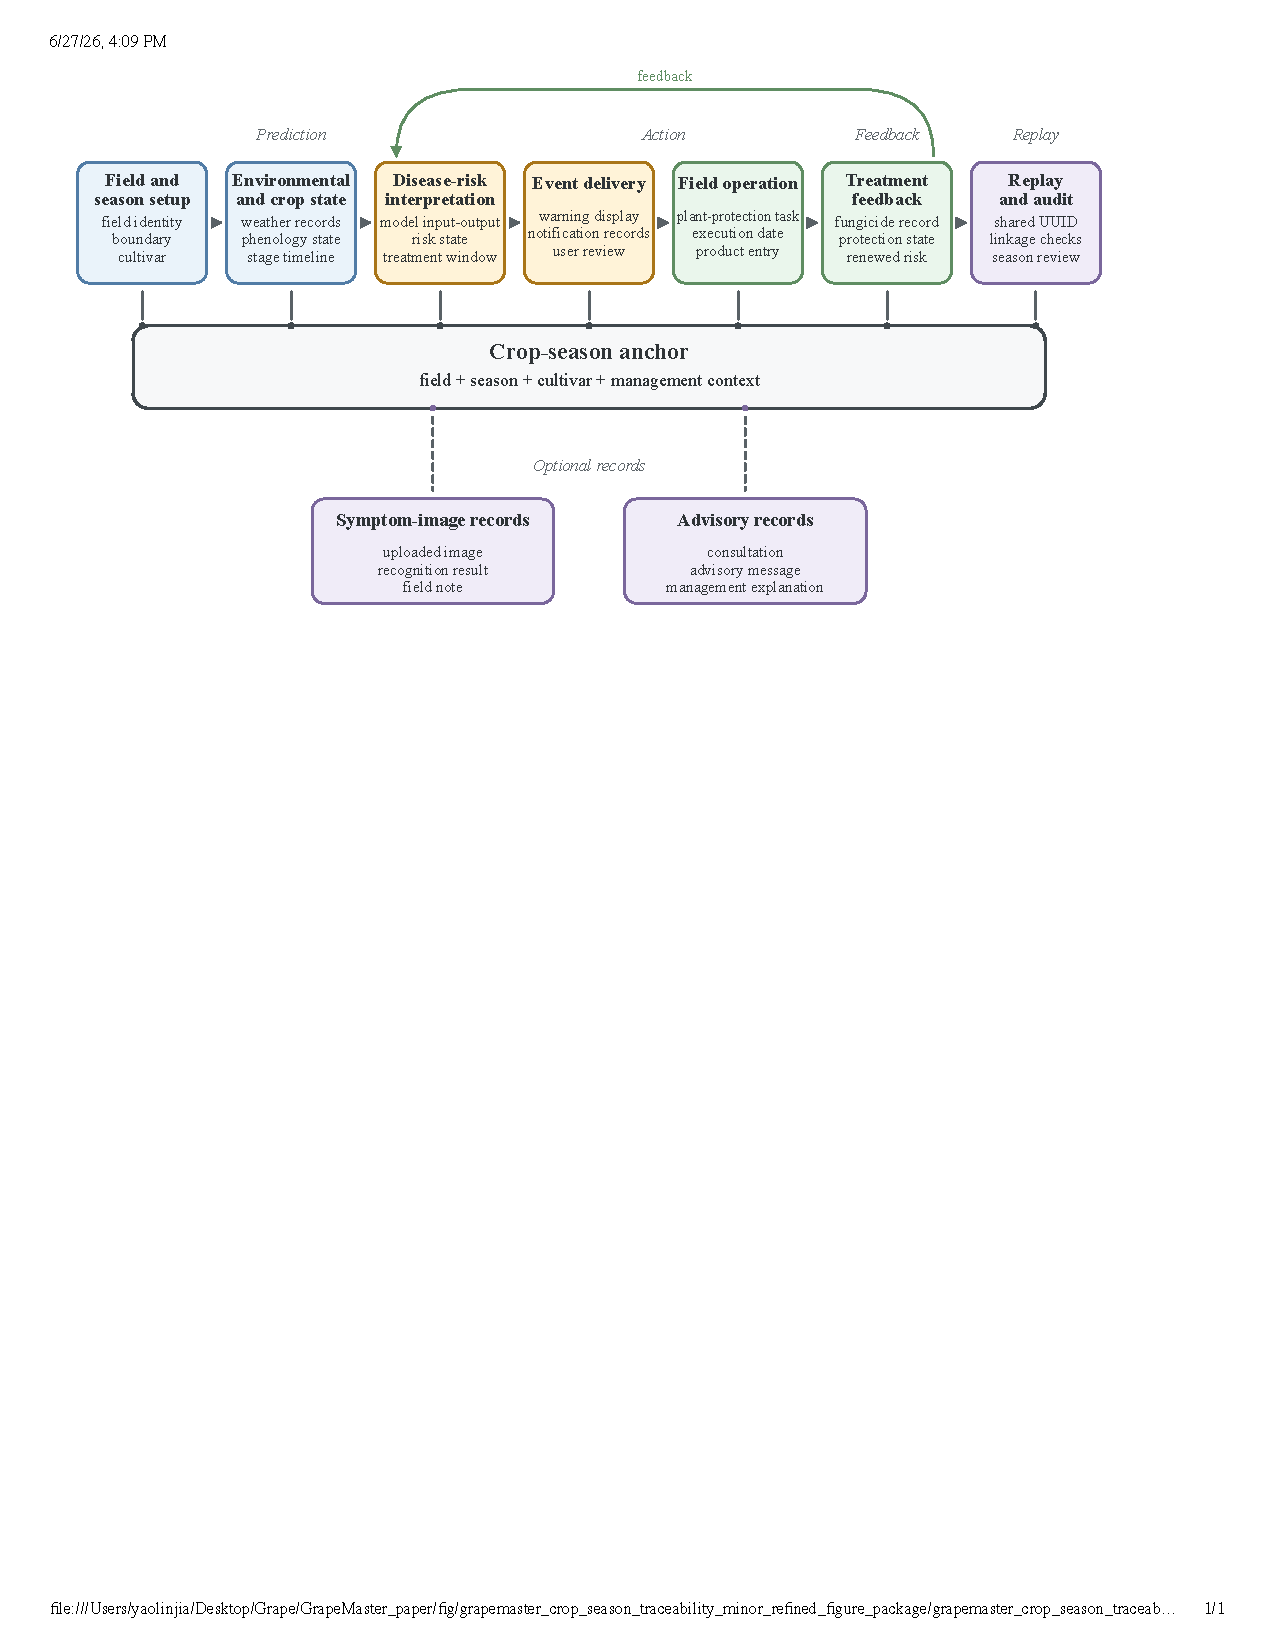
\includegraphics[width=\linewidth]{../fig/grapemaster_crop_season_traceability_minor_refined_figure_package/grapemaster_crop_season_traceability_minor_refined.pdf}
\caption[Crop-season-centered traceability architecture]{Crop-season-centered traceability architecture implemented in GrapeMaster. The crop season serves as the platform management unit linking field setup, environmental and crop state, disease-risk interpretation, event delivery, field operation, treatment feedback, optional symptom and advisory evidence, and replay/audit records. The feedback path indicates that completed plant-protection records can update later protection-state or risk interpretation, while replay/audit records support reconstruction of the prediction--action--feedback chain.}
\label{fig:crop_season_traceability_architecture}
\end{figure}

\subsection{Weather ingestion and crop-season preprocessing}\label{weather-ingestion-and-crop-season-preprocessing}

For each active crop season, scheduled workflows retrieve historical and forecast weather using the field location. The weather workflow combines historical observations with forecast records where available. Hourly and daily variables include temperature, humidity, dew-point or wetness-related variables, precipitation, wind conditions, and daily summary variables. Missing values are handled before analytical use so that downstream workflows receive complete date-aligned input series.

The backend transforms weather data into three working schemas. Daily mean temperature is converted into phenology-model input; hourly weather is converted into the disease-model schema, including datetime, dew point, precipitation, relative humidity, air temperature, and wind speed; and short-term hourly records are used to evaluate spraying suitability. This preprocessing belongs to the GrapeMaster platform workflow and defines the input schema required by the platform-compatible analytical modules.

\subsection{Platform-compatible analytical modules and module-level evaluation}\label{analytical-modules-operationalized-in-grapemaster}

\subsubsection{Phenology simulation and Guangxi calibration}\label{phenology-simulation-and-guangxi-calibration}

The phenology workflow estimates grapevine growth-stage progression from daily temperature and crop-season metadata. The backend calculates daily thermal accumulation and maps accumulated development to broad BBCH-related growth-stage classes. The output provides a crop-development timeline for mobile display and a daily crop-stage sequence for disease-risk interpretation, warning windows, and management-task scheduling.

For regional evaluation, Guangxi field phenology observations were mapped to broad major-stage classes: early season or budburst, leaf development, inflorescence emergence, flowering, berry development, ripening, and post-harvest or senescence. Daily mean temperature was converted to cumulative thermal progress after a meteorological biofix:
\begin{equation}
\mathrm{GDD}_{t}
=
\sum_{d=1}^{t} f_{\mathrm{WE}}\left(T_{d}\right),
\label{eq:phenology_gdd}
\end{equation}
where \(T_d\) is daily mean temperature and \(f_{\mathrm{WE}}(\cdot)\) is the Wang--Engel temperature-response function. The accumulated value was mapped to the broad-stage sequence using cultivar-specific major-stage thresholds. For mobile display, the predicted major stage was supplemented with within-stage progress and a transition label when the thermal state was close to an adjacent stage boundary.

The Guangxi observations were evaluated using grouped validation by site-year and cultivar-stratified grouping where possible. The primary metrics were exact major-stage agreement, user-visible agreement after transition-window display, adjacent-stage agreement, severe misclassification rate, and mean absolute stage distance. The cultivar wk was represented by one sparse site-year and was reported separately.

\subsubsection{FSIM-S downy mildew first-infection risk engine}\label{fsim-s-downy-mildew-first-infection-risk-engine}

The disease-risk service receives weather, crop-stage sequence, cultivar susceptibility, target disease information, and fungicide-history inputs through the platform interface. It returns date-aligned disease-risk states, field-risk states, protection states, recommendations, and treatment windows.

For GrapeMaster, the disease-risk module was configured with FSIM-S, a first seasonal infection model developed for humid subtropical grape-growing areas in Guangxi. The module predicts the first seasonal infection of grapevine downy mildew under conditions where early-season infection may be driven by recurrent airborne asexual sporangia rather than by a discrete oospore-driven primary infection event. It was calibrated and validated using 2022--2024 site-year observations from Guangxi, including phenology, airborne sporangia, symptom onset, management records, and meteorological data.

FSIM-S uses a mechanistic infection chain adapted from Rossi primary-infection modelling and related sporangia-based infection modelling work \citep{rossiMechanisticModelSimulating2008,caffiModelPredictingPrimary2009c,caffiEvaluationDynamicModel2011,brischettoWeatherDrivenModelPredicting2021}. In the subtropical setting, airborne sporangia are treated as the relevant inoculum source for the first seasonal infection, and the model represents the main steps from sporangia availability and deposition to infection establishment, incubation, and symptom expression.

The FSIM-S configuration evaluated in this study uses field-derived spore pressure to regulate the infection-triggering threshold. A daily sporangia pressure field \(S(d)\) is constructed from field spore monitoring data after interpolation, normalization, and smoothing. Hourly pressure is represented as a three-day rolling mean:
\begin{equation}
P_{t}
=
\frac{1}{3}
\sum_{k=0}^{2} S\left(d_{t}-k\right),
\label{eq:spore_pressure}
\end{equation}
where \(P_t\) is the spore-pressure index at hour \(t\), and \(d_t\) is the corresponding calendar day.

Infection is triggered when the wetness-duration term and its temperature response exceed a spore-pressure-adjusted effective threshold:
\begin{equation}
\begin{array}{l@{\;}c@{\;}l}
\displaystyle \mathrm{IC}_t^{*}
&=&
\displaystyle
\begin{cases}
\mathrm{IC}\exp\left(-\alpha_{\mathrm{pos}}P_t\right),
& P_t \geq 0,\\[2pt]
\mathrm{IC}\exp\left[\alpha_{\mathrm{neg}}\left(-P_t\right)\right],
& P_t < 0,
\end{cases}\\[8pt]
\displaystyle \mathrm{infection}_t
&=&
\displaystyle \mathbb{I}\left(\mathrm{WD}_t\,\mathrm{TWD}_t \geq \mathrm{IC}_t^{*}\right),
\end{array}
\label{eq:fsims_threshold}
\end{equation}
where \(\mathrm{WD}_t\) is the wetness-duration component, \(\mathrm{TWD}_t\) is the temperature response during the wetness period, \(\mathrm{IC}\) is the base infection threshold, \(\alpha_{\mathrm{pos}}\) and \(\alpha_{\mathrm{neg}}\) are calibration parameters for positive and negative spore-pressure effects, and \(\mathbb{I}(\cdot)\) is an indicator function. Positive spore pressure lowers the effective infection threshold, whereas low pressure raises it.

The disease-risk workflow was limited to downy mildew because FSIM-S was calibrated for this target disease. Other grape diseases were represented in image-recognition or advisory functions but were not disease-risk prediction targets in this study. Weather inputs can be supplied through public weather services, grid weather products, regional weather data, local weather stations, or other sources that can be transformed into the platform schema. The spore-pressure term represents an FSIM-S model-level enhancement and an optional sensor-enhanced pathway for vineyards that deploy spore-trapping equipment; it was not required as a live input for routine platform operation.

Supplementary Figure S1 presents the platform-level inputs, transformations, and user-facing outputs required for integrating the disease-risk engine with the GrapeMaster workflow.

\subsubsection{Grape disease recognition and LLM-assisted advisory}\label{grape-disease-recognition-and-bounded-llm-advisory}

The image-based workflow supports symptom-level evidence after disease signs are observed or suspected. Users can upload field images through the mobile client, and the image-recognition service returns disease or healthy categories with associated diagnostic or management text for display. Image outputs can be linked to crop-season notes, disease reports, and advisory records, allowing visual evidence to remain within the same crop-season context as other management records.

The image-recognition and advisory module follows the published CDIP-ChatGLM3 dual-model framework, which combines a deep-learning image classifier with a fine-tuned ChatGLM3-based advisory model for crop disease identification and management guidance \citep{yanCDIPChatGLM3DualmodelApproach2025}. In this study, the framework was adapted to the grape scenario by expanding the grape disease image dataset with additional field photographs and two grape disease categories. The platform-compatible visual model was selected according to grape-focused validation performance.

For image recognition, each candidate model outputs class probabilities using a softmax layer and is trained with cross-entropy loss:
\begin{equation}
\begin{array}{l@{\;}c@{\;}l}
\displaystyle p\left(y=k\mid x\right)
&=&
\displaystyle \frac{\exp\left(z_k\right)}
{\sum_{j=1}^{K}\exp\left(z_j\right)},\\[4pt]
\displaystyle \mathcal{L}_{\mathrm{CE}}
&=&
\displaystyle -\sum_{k=1}^{K}y_k
\log p\left(y=k\mid x\right),
\end{array}
\label{eq:softmax}
\end{equation}
where \(x\) is the input image, \(z_k\) is the logit for disease class \(k\), \(K\) is the number of grape disease or healthy categories, and \(y_k\) is the one-hot class label. Model selection is based on grape-focused validation metrics, including accuracy, precision, recall, and F1-score:
\begin{equation}
m^{*}
=
\arg\max_{m\in\mathcal{M}}
\mathrm{Score}_{\mathrm{val}}\left(m\right),
\label{eq:model_selection}
\end{equation}
where \(\mathcal{M}\) is the set of candidate vision models and \(\mathrm{Score}_{\mathrm{val}}\) is the selected validation criterion, such as accuracy or macro-F1. The selected classifier provides the disease label and confidence score used by the advisory interface.

The LLM-assisted advisory component follows the CDIP-ChatGLM3 interaction structure: image-recognition outputs are converted into disease-specific consultation context, and the fine-tuned language model generates management-oriented advisory text. In the platform workflow, LLM messages and advisory outputs are stored or linked to the crop-season context where possible. Supplementary Figure S2 summarizes the image-recognition and advisory workflow.

\subsection{Module provenance and evidence boundaries}\label{module-provenance-and-operationalization-table}

\begin{table}[H]
\centering
\caption[Provenance and evidence boundaries of GrapeMaster components]{Provenance, platform roles, and evidence boundaries of the main GrapeMaster components. Backend records and module-level evidence are reported separately because they support different claim levels.}
\label{tab:module_provenance}
\tablefontsize
\begin{tabular}{@{}p{0.18\linewidth} p{0.22\linewidth} p{0.24\linewidth} p{0.24\linewidth}@{}}
\toprule
Module & Source or provenance & Platform role & Evidence and boundary \\
\midrule
Platform workflow & Deployed GrapeMaster backend, mobile client, database, scheduled jobs, and notification/task services & Links field, crop season, weather, phenology, risk, task, fungicide, image, advisory, and record objects & Deployed-platform evidence for workflow operability and data linkage; not evidence of production effects \\
Phenology module & Weather-driven phenology workflow calibrated with Guangxi field observations & Crop-stage timing for risk interpretation, advisory timing, and task scheduling & Offline module-level evidence for platform-compatible broad-stage crop context \\
FSIM-S risk engine & Team-developed downy mildew first-infection model calibrated and validated with Guangxi field data & First seasonal infection-period warning for task triggering and protection-state interpretation & Offline module-level evidence for a platform-compatible downy mildew risk component \\
Grape disease recognition & Platform-compatible grape disease visual model based on the published CDIP-ChatGLM3 framework & Post-symptomatic image evidence and disease category output & Offline validation evidence for a platform-compatible grape disease image component \\
LLM advisory & Fine-tuned ChatGLM3-based advisory model from the CDIP-ChatGLM3 framework & Consultation, explanation, and agronomic advisory text & Knowledge-support evidence for grape disease consultation cases; does not replace expert or regulatory decisions \\
\bottomrule
\end{tabular}
\end{table}

\begin{table}[H]
\centering
\caption{Evidence-to-claim boundaries used in the GrapeMaster evaluation.}
\label{tab:evidence_claim_boundary}
\tablefontsize
\begin{tabular}{@{}p{0.26\linewidth} p{0.34\linewidth} p{0.30\linewidth}@{}}
\toprule
Evidence source & Supported claim & Boundary or excluded claim \\
\midrule
Deployed backend records & GrapeMaster generated linked crop-season, weather, phenology, risk, notification, task, fungicide, image, advisory, and record objects in the operational database & Does not prove post-replacement module performance, user adoption, pesticide reduction, disease-control efficacy, or economic benefit \\
Offline module-level validation & The FSIM-S, broad-stage phenology, and grape disease image-recognition components have platform-compatible inputs, outputs, and module-level analytical evidence for the Guangxi context & Does not represent full-season production validation after replacing or updating modules in the deployed platform \\
Representative crop-season replay & A selected crop-season management unit can retrieve weather, phenology, disease-risk, notification, task, and fungicide records as a traceable risk-to-feedback chain & Does not represent population-level behaviour or a controlled agronomic outcome test \\
\bottomrule
\end{tabular}
\end{table}

\subsection{Risk-task-protection workflow and evaluation boundaries}\label{closed-loop-workflow-and-evaluation-boundaries}

\subsubsection{Risk-task-protection feedback logic}\label{risk-task-protection-feedback-logic}

The risk-task-protection workflow starts from the daily disease-risk output generated for an active crop season. The platform translates model output into user-facing risk states, such as protected, low-risk, favourable, or high-risk periods. When weather, phenology, and disease-risk outputs indicate a favourable infection window, the crop-season page and notification interface display the corresponding risk state and prompt the user to review the field condition and treatment window.

The notification is linked to the crop season rather than to a stand-alone warning message. From the warning page, the user can enter the plant-protection workflow, inspect the suggested treatment timing, and create a plant-protection task if intervention is required. This design connects risk viewing, decision review, and task creation within the same crop-season context.

After a plant-protection task is created, the user can keep it pending, complete it after field operation, or leave it unexecuted. A completed task records the execution date and pesticide or fungicide information and is then used by the platform as management feedback. This rule follows the practical plant-protection assumption that fungicide applications can provide a temporary protection window whose duration depends on product properties, application timing, host growth, rainfall, and disease pressure \citep{caffiFungicideModelsAre2018,bleyerTogetherBetterImprovement2020,oliverFungicideUsePatterns2023,warnekeEffectFungicideMobility2020}. In this workflow, a completed fungicide-related task activates a rule-based protection period or low-risk management state. During this period, the crop-season risk display is updated to a protected or low-risk state.

When the protection period ends, the platform resumes dynamic risk prediction using the updated weather, phenology, disease-risk input, and management history. If a new favourable or high-risk window appears, the system again displays the risk state and prompts the user to review the need for a new plant-protection task. The resulting cycle is: risk prediction, risk-state display, user notification, task creation, task completion, protected-state update, and renewed risk prediction.

The image-recognition and LLM-assisted advisory modules provide an additional entry point when users observe symptoms during the crop season. A user can upload a field image for disease identification, and the platform returns a grape-disease diagnosis result that can be reviewed together with the current crop-season risk state. For downy mildew, this image-based confirmation can be aligned with the risk-prediction workflow. For other supported grape diseases, such as powdery mildew, the module provides diagnostic support without being treated as an equivalent risk-forecasting workflow.

The LLM-assisted function is positioned as a supplementary advisory and knowledge-support channel. Within the crop-season context, it supports agronomic consultation, interpretation of recognition results, and communication of standard management guidance. Risk forecasting and image-based disease diagnosis remain handled by the dedicated analytical modules; LLM outputs are treated as auxiliary information for learning, communication, and management planning rather than as a replacement for validated models, expert diagnosis, pesticide labels, or local regulations.

\subsubsection{Backend records, crop-season replay, and evaluation boundaries}\label{backend-records-crop-season-replay-and-evaluation-boundaries}

Backend database exports from GrapeMaster were used to assess whether the platform had generated the record types required by the workflow. The exported tables included user and profile tables, field records, crop-season records, notifications, plant-protection tasks, irrigation tasks, fungicide and pesticide records, weather-related records, phenology records, disease-risk records, image-recognition and advisory records, disease-report records, note records, and message records. These tables were treated as operational records for evaluating workflow operability and traceability.

Account-level screening was applied before summarizing GrapeMaster records. Accounts without business records or without both field and crop-season records were excluded because they could not support a crop-season-centered workflow. One non-target-region account was also removed from the vineyard evaluation set. Detailed screening rules are listed in Supplementary Table S8. After screening, 47 accounts remained from 95 deduplicated accounts and were used as the candidate account set for describing GrapeMaster operational-record coverage.

The screened records were used for four workflow checks: field and crop-season creation and linkage; attachment of weather, phenology, risk, and notification records to crop seasons; creation and status updating of plant-protection tasks and pesticide/fungicide records; and linkage of image, advisory, disease-report, and note records to management contexts.

The representative replay anchor was selected as a chain-complete audit case from retained crop seasons that had the minimum traceability chain required for risk-to-feedback reconstruction: linked weather, phenology, disease-risk or request-response payloads, notification records, completed plant-protection tasks, and fungicide-product records. The replay was not selected to estimate population-level user behaviour, task-completion frequency, agronomic efficacy, pesticide reduction, or adoption rate. It was used to test whether the expected workflow objects could be reconstructed through shared crop-season or task identifiers and whether any expected evidence object was absent under the selected anchor.

The study uses separate evidence sources for platform workflow records and analytical modules. The screened backend records and workflow outputs were used to evaluate field creation, crop-season management, weather and phenology records, disease-risk output, notification delivery, plant-protection task handling, fungicide-feedback logic, image upload, LLM consultation, and management-record storage. Module-level evidence was evaluated separately for the downy mildew initial-infection model, phenology module, grape disease image-recognition module, and LLM advisory module. The resulting evidence therefore supports deployed workflow operability, record traceability, representative crop-season replay, and module-level analytical readiness. It does not evaluate post-replacement full-season production performance, user adoption, pesticide reduction, disease-control efficacy, or economic outcomes.

\section{Results}\label{results}

\subsection{Backend-record evidence for crop-season-centered linkage}\label{deployed-platform-architecture-and-operational-data-coverage}

The cleaned GrapeMaster backend export contained 95 deduplicated registered accounts. Among them, 47 accounts contained both field records and crop-season records; the remaining 48 accounts did not contain field-crop-season linkage data.

Within the 47 accounts with field-crop-season linkage, the backend contained 139 vineyard fields and 128 crop seasons. Analytical-state records were linked at the crop-season level, including 126 weather payloads, 126 phenology payloads, and 252 disease-risk or model request-response payloads. Event and operation records were also retained, including 3590 notifications, 151 plant-protection or irrigation tasks, and 234 fungicide or pesticide records.

The optional evidence branches contained 94 field-note or disease-report records, 2808 image-analysis records, 1360 advisory or message records, and 27 forum records. Figure~\ref{fig:backend_operational_linkage} summarizes the backend linkage among these retained record classes. Table~\ref{tab:backend_operational_coverage} reports the corresponding linkage evidence and result boundaries.

\begin{figure}[H]
\centering
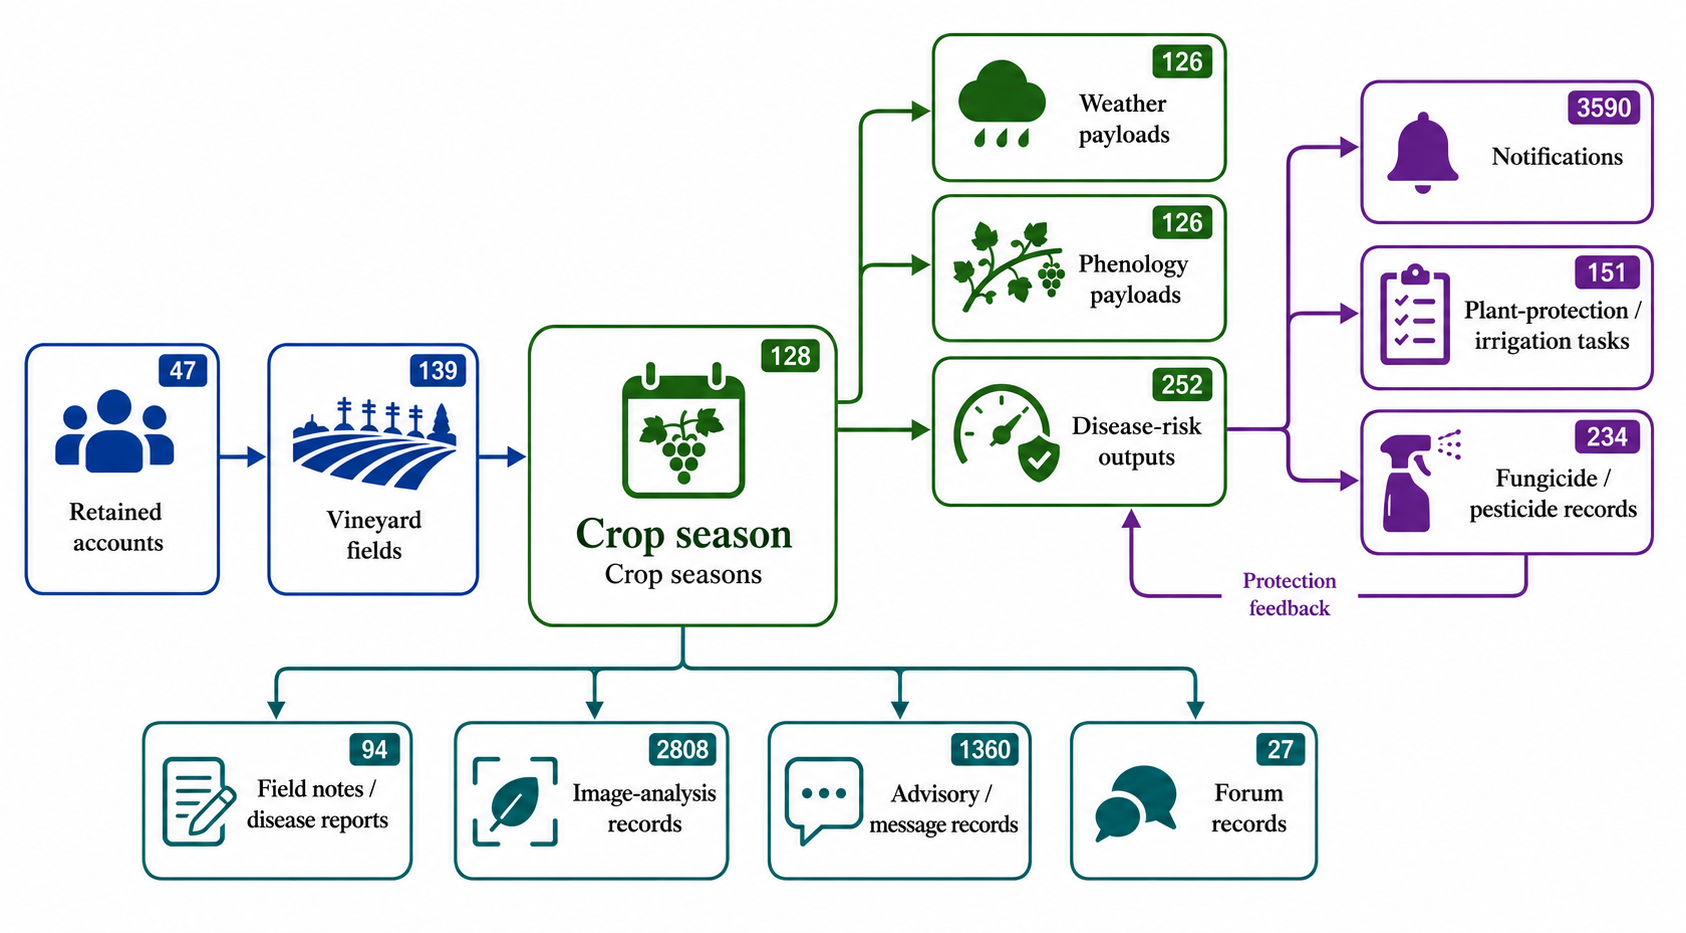
\includegraphics[width=\linewidth]{../fig/grapemaster_backend_linkage.png}
\caption[Architecture-level backend linkage among retained GrapeMaster records]{Architecture-level backend linkage among retained GrapeMaster records. The crop-season record is shown as the central anchor connecting account-field setup, analytical payloads, risk outputs, notifications, tasks, protection feedback, image-analysis records, advisory messages, and forum records.}
\label{fig:backend_operational_linkage}
\end{figure}

\begin{table}[H]
\centering
\begingroup
\setlength{\tabcolsep}{3pt}
\renewcommand{\arraystretch}{1.12}
\scriptsize
\caption{Backend-record evidence for crop-season-centered linkage in the retained GrapeMaster export.}
\label{tab:backend_operational_coverage}
\begin{tabular}{p{0.21\linewidth} p{0.30\linewidth} p{0.22\linewidth} p{0.18\linewidth}}
\toprule
Evidence level & Retained records & Linkage basis & Result supported \\
\midrule
Screened workflow set & 47 of 95 deduplicated accounts retained after screening & At least one field and one crop season & Accounts available for crop-season workflow evaluation \\
Field-season denominator & 139 fields and 128 crop seasons & Retained account, field UUID, and crop-season UUID & Field and crop-season records established as the verification base \\
Crop-season state records & 126 crop seasons with linked weather, phenology, risk, and request-response payloads & Shared crop-season UUID & Environmental, crop-stage, and disease-risk states reconstructable by crop season \\
Event and operation records & 3590 notifications and 151 plant-protection or irrigation tasks & Retained user, field, or crop-season context & Event-delivery and field-operation records retained \\
Treatment-feedback records & 234 fungicide or pesticide records linked to 141 plant-protection tasks & Task UUID & Product records connected to completed or recorded task contexts \\
Symptom and advisory records & 94 field-note or disease-report records, 2808 image-analysis records, 1360 advisory or message records, and 27 forum records & Account, field, crop-season, image, or message identifiers & Optional evidence branches retained; completeness varies by season \\
Claim boundary & No controlled production comparison in the backend export & Not applicable & No efficacy, pesticide-reduction, adoption, or economic outcome inferred \\
\bottomrule
\end{tabular}
\endgroup
\end{table}

\subsection{Crop-season workspace and analytical-state display}\label{crop-season-centered-data-linkage-and-mobile-workflow-implementation}

The mobile client displayed vineyard fields and crop seasons as the entry points for management functions. Field-management pages provided field creation, inspection, selection, sharing, deletion, recovery, crop-season access, and links to weather, phenology, disease-risk warning, notifications, tasks, notes, and image-related records (Supplementary Figure S3).

Weather and phenology outputs were displayed within the selected crop-season workspace. The weather page presented near-term field-specific weather information (Figure~\ref{fig:weather_phenology_interfaces_result}a). The operation-timing page displayed hourly weather conditions and spray-suitability information for field work planning (Figure~\ref{fig:weather_phenology_interfaces_result}b). The crop-season workspace summarized field-risk and growth-stage states under the selected field context (Figure~\ref{fig:weather_phenology_interfaces_result}c).

The displayed workspace was consistent with the backend linkage result in Table~\ref{tab:backend_operational_coverage}: weather and phenology payloads were retrieved as crop-season state information rather than as detached model outputs.

\begin{figure}[H]
\centering
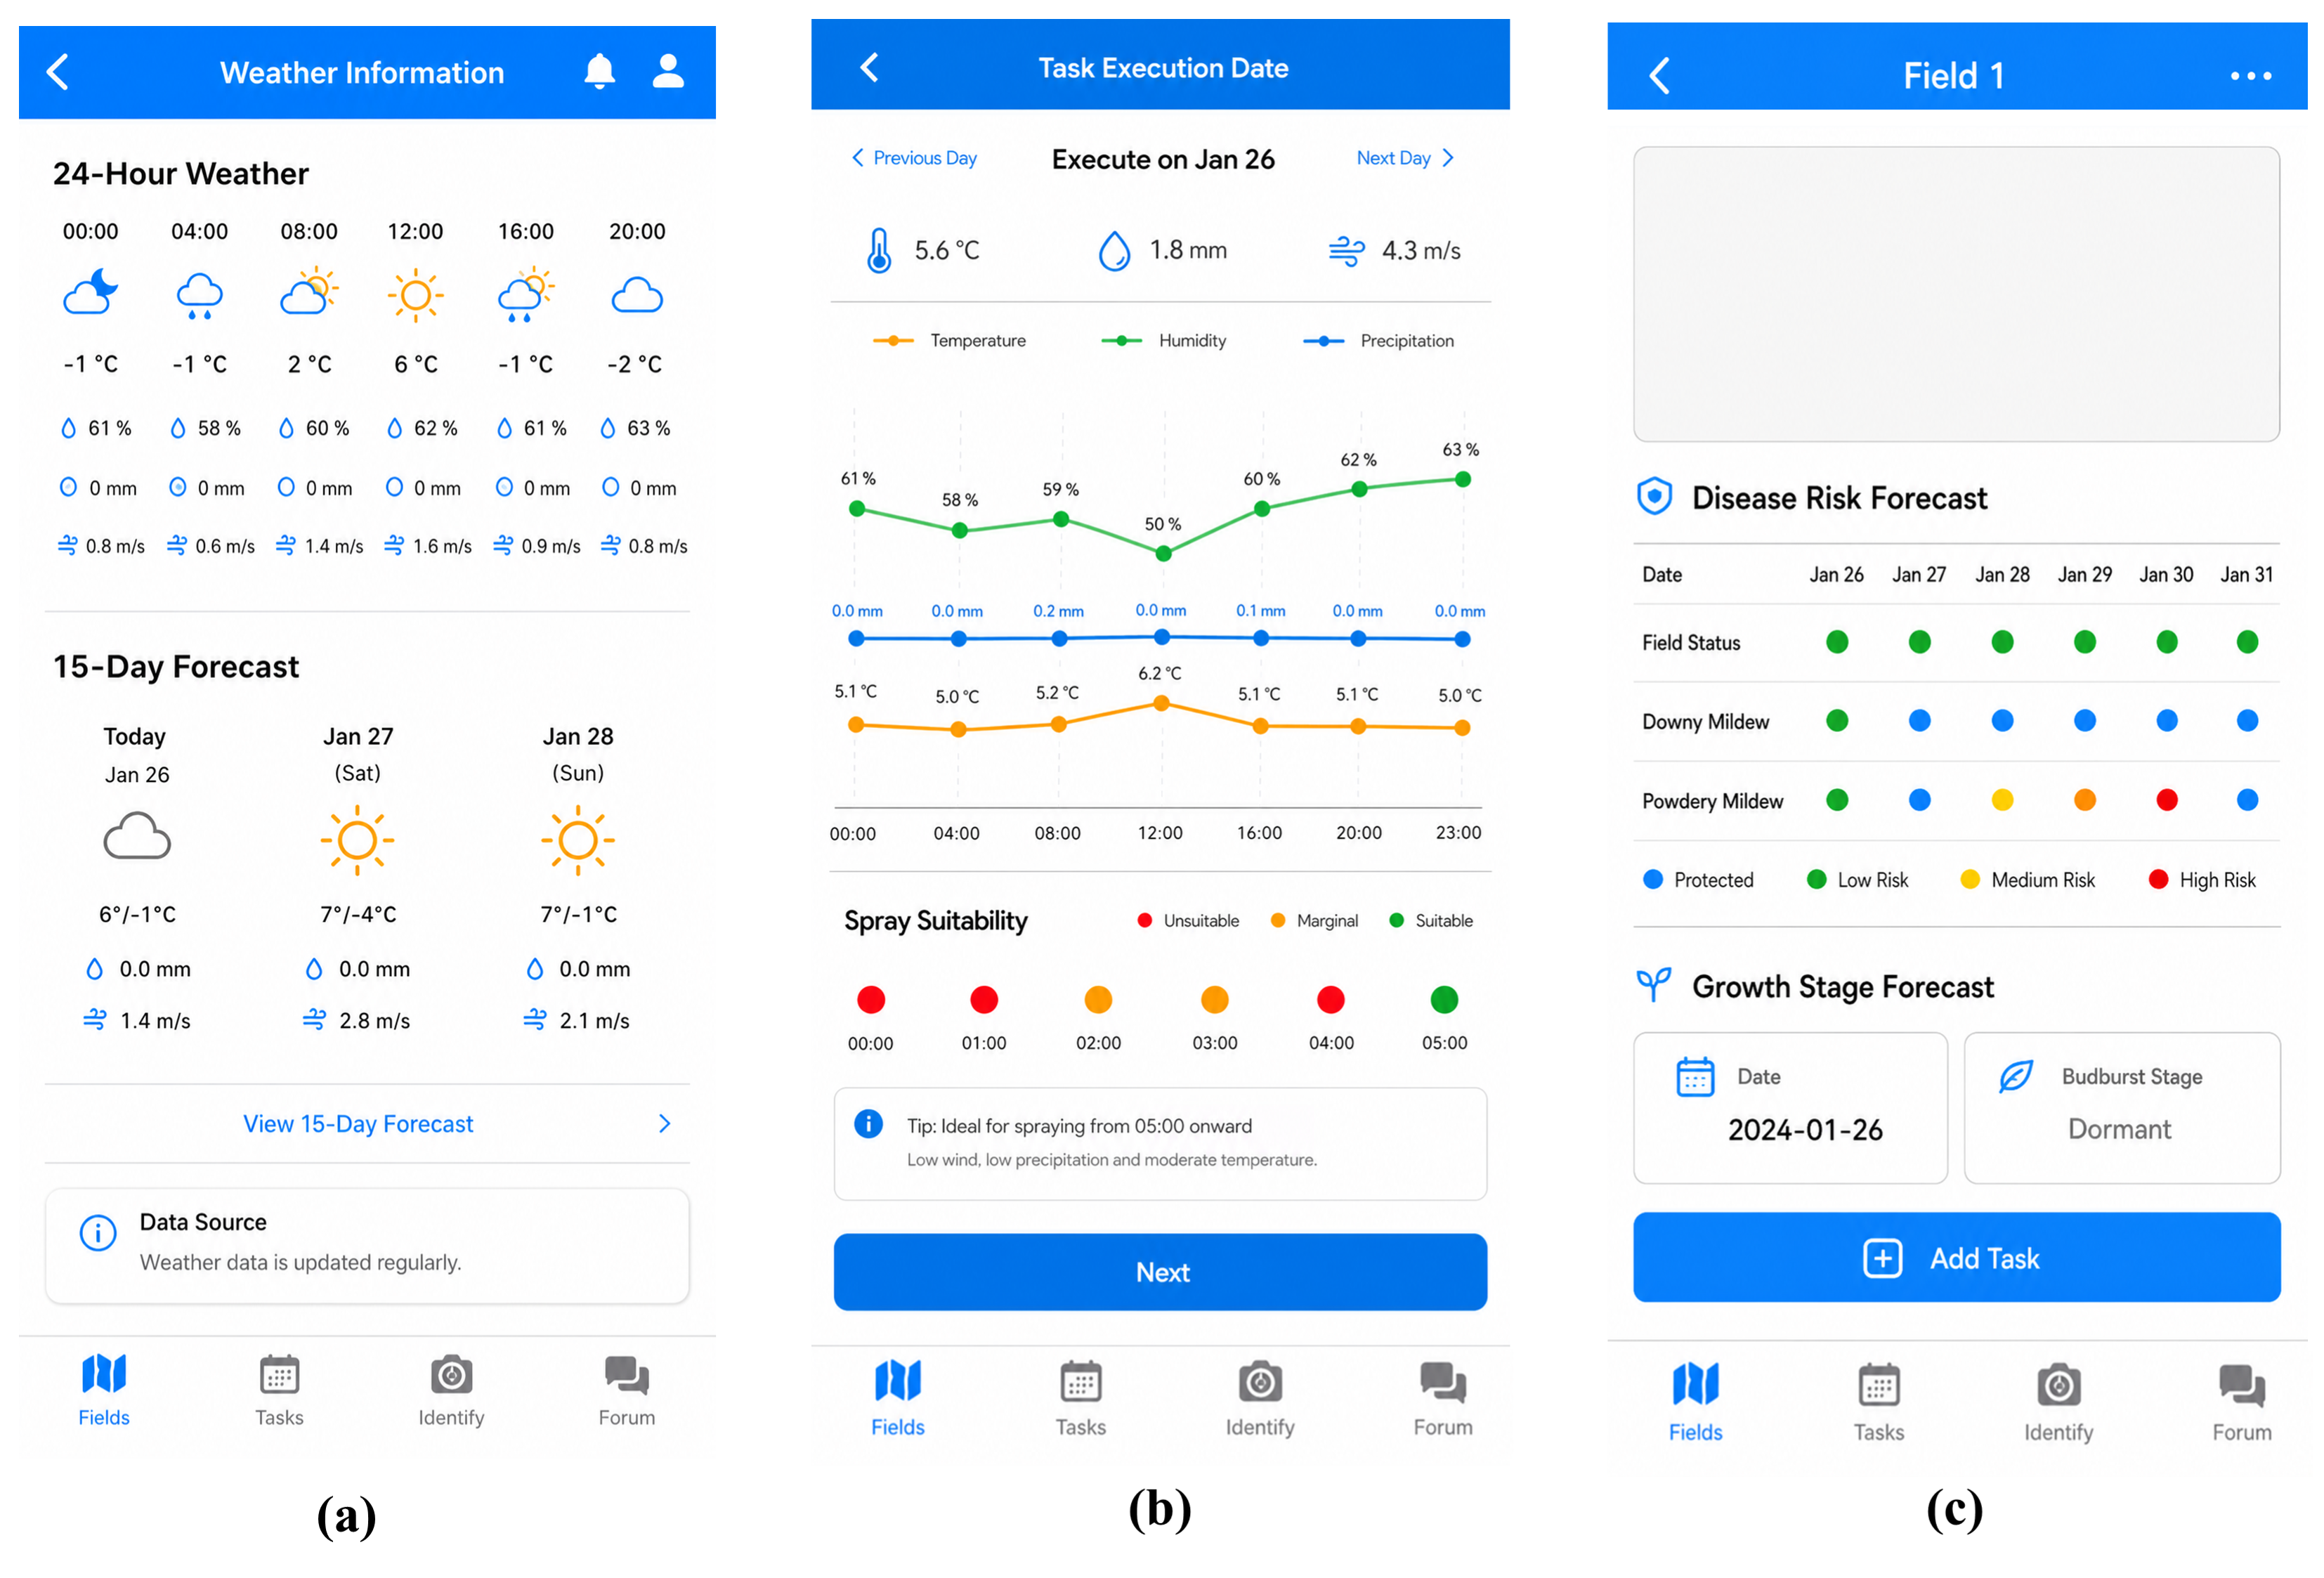
\includegraphics[width=\linewidth]{../fig/weather_phenology_interfaces.png}
\caption[Crop-season workspace for weather and phenology state]{Crop-season workspace for weather and phenology state in GrapeMaster. (a) The weather page displays near-term field-specific weather information. (b) The operation-timing page displays hourly weather and spray-suitability information. (c) The crop-season workspace displays field-risk and growth-stage summaries under the selected field context.}
\label{fig:weather_phenology_interfaces_result}
\end{figure}

\subsection{Risk delivery, operation feedback, and evidence capture}\label{risk-delivery-operation-feedback-and-evidence-capture}

Disease-risk outputs were displayed as a date-aligned mobile timeline for crop-season review. The timeline presented downy mildew risk together with field-level risk states in the Mingyang crop-season case (Figure~\ref{fig:disease_risk_timeline_result}a), in a Guangxi crop-season case without fungicide-feedback records (Figure~\ref{fig:disease_risk_timeline_result}b), and in the same case after fungicide-feedback records were included (Figure~\ref{fig:disease_risk_timeline_result}c).

The warning and notification interfaces displayed crop-season and disease-risk events as reviewable mobile records. The disease-alert dialog displayed a disease-risk event (Figure~\ref{fig:alert_notification_interfaces_result}a), the management-notice dialog displayed a task-related prompt (Figure~\ref{fig:alert_notification_interfaces_result}b), and the notification list retained reviewable event records (Figure~\ref{fig:alert_notification_interfaces_result}c). These notification records corresponded to the retained event-delivery records summarized in Table~\ref{tab:backend_operational_coverage}.

Task interfaces recorded field-operation information after crop-season events were reviewed. The task list displayed field-operation records and status (Figure~\ref{fig:task_management_interfaces_result}a), the product-selection page retained fungicide or pesticide entries linked to plant-protection tasks (Figure~\ref{fig:task_management_interfaces_result}b), and the in-tank mixing page recorded sprayer capacity, product dosage, plot area, water volume, and planned date (Figure~\ref{fig:task_management_interfaces_result}c).

The image-based disease-assistance interfaces displayed symptom-image upload (Figure~\ref{fig:ai_diagnosis_interfaces_result}a), disease-recognition output (Figure~\ref{fig:ai_diagnosis_interfaces_result}b), and advisory interaction functions (Figure~\ref{fig:ai_diagnosis_interfaces_result}c). These records corresponded to the image-analysis and advisory/message evidence branch reported in Table~\ref{tab:backend_operational_coverage}.

\begin{figure}[H]
\centering
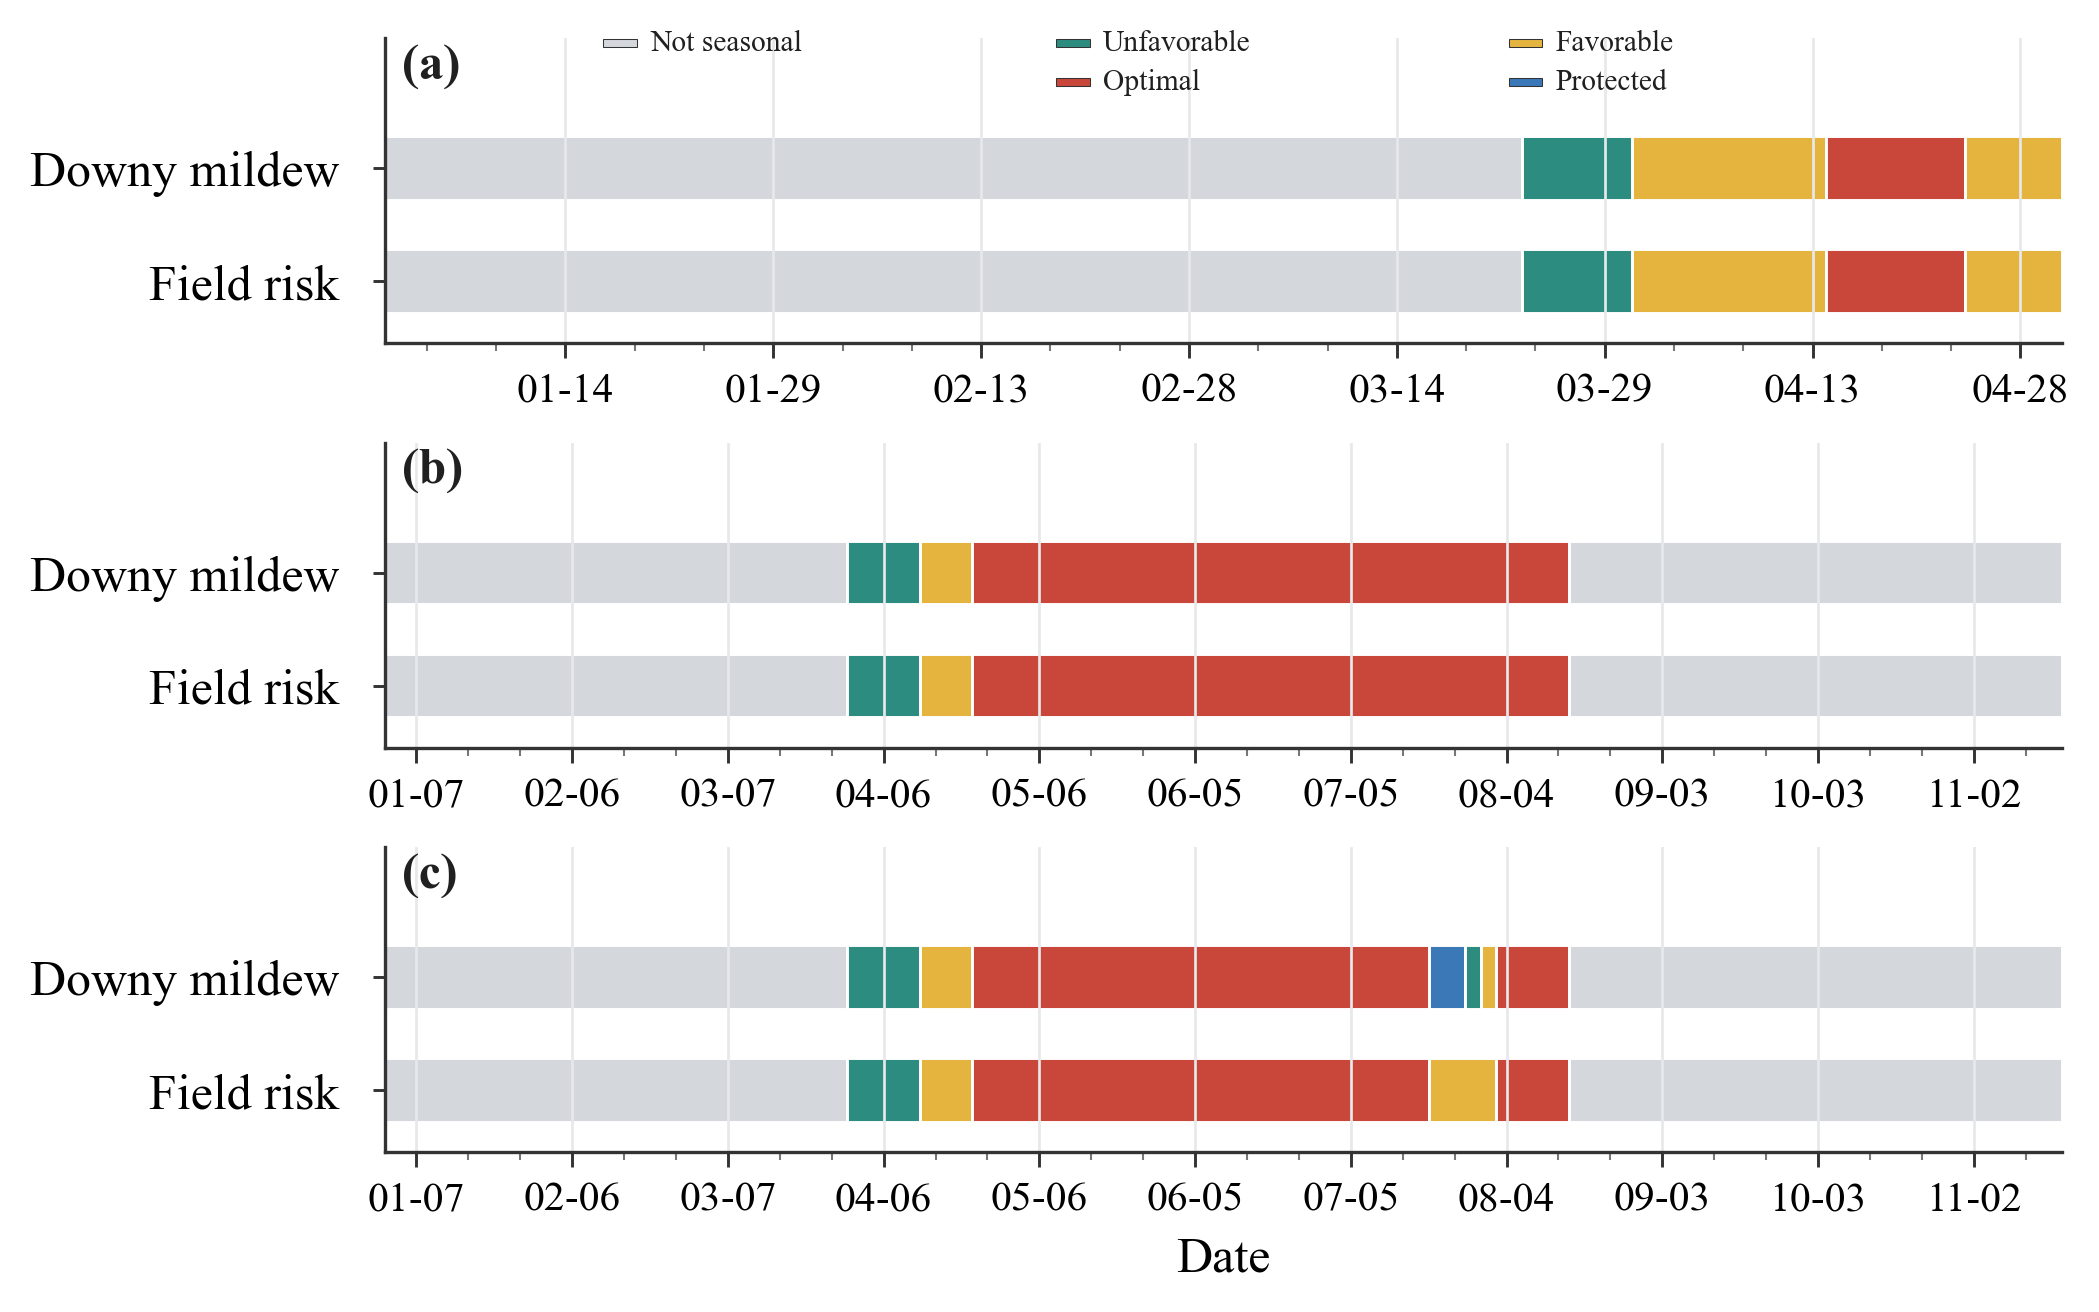
\includegraphics[width=\linewidth]{../fig/disease_risk_timeline_downy_field.png}
\caption[Disease-risk timeline in the GrapeMaster mobile workflow]{Disease-risk timeline in the GrapeMaster mobile workflow. (a) Mingyang 2024 shows date-aligned downy mildew and field-risk states. (b) A Guangxi crop-season case without fungicide-feedback records shows the untreated risk-state sequence. (c) The same Guangxi crop-season case with fungicide-feedback records shows the corresponding protected-state updates.}
\label{fig:disease_risk_timeline_result}
\end{figure}

\begin{figure}[H]
\centering
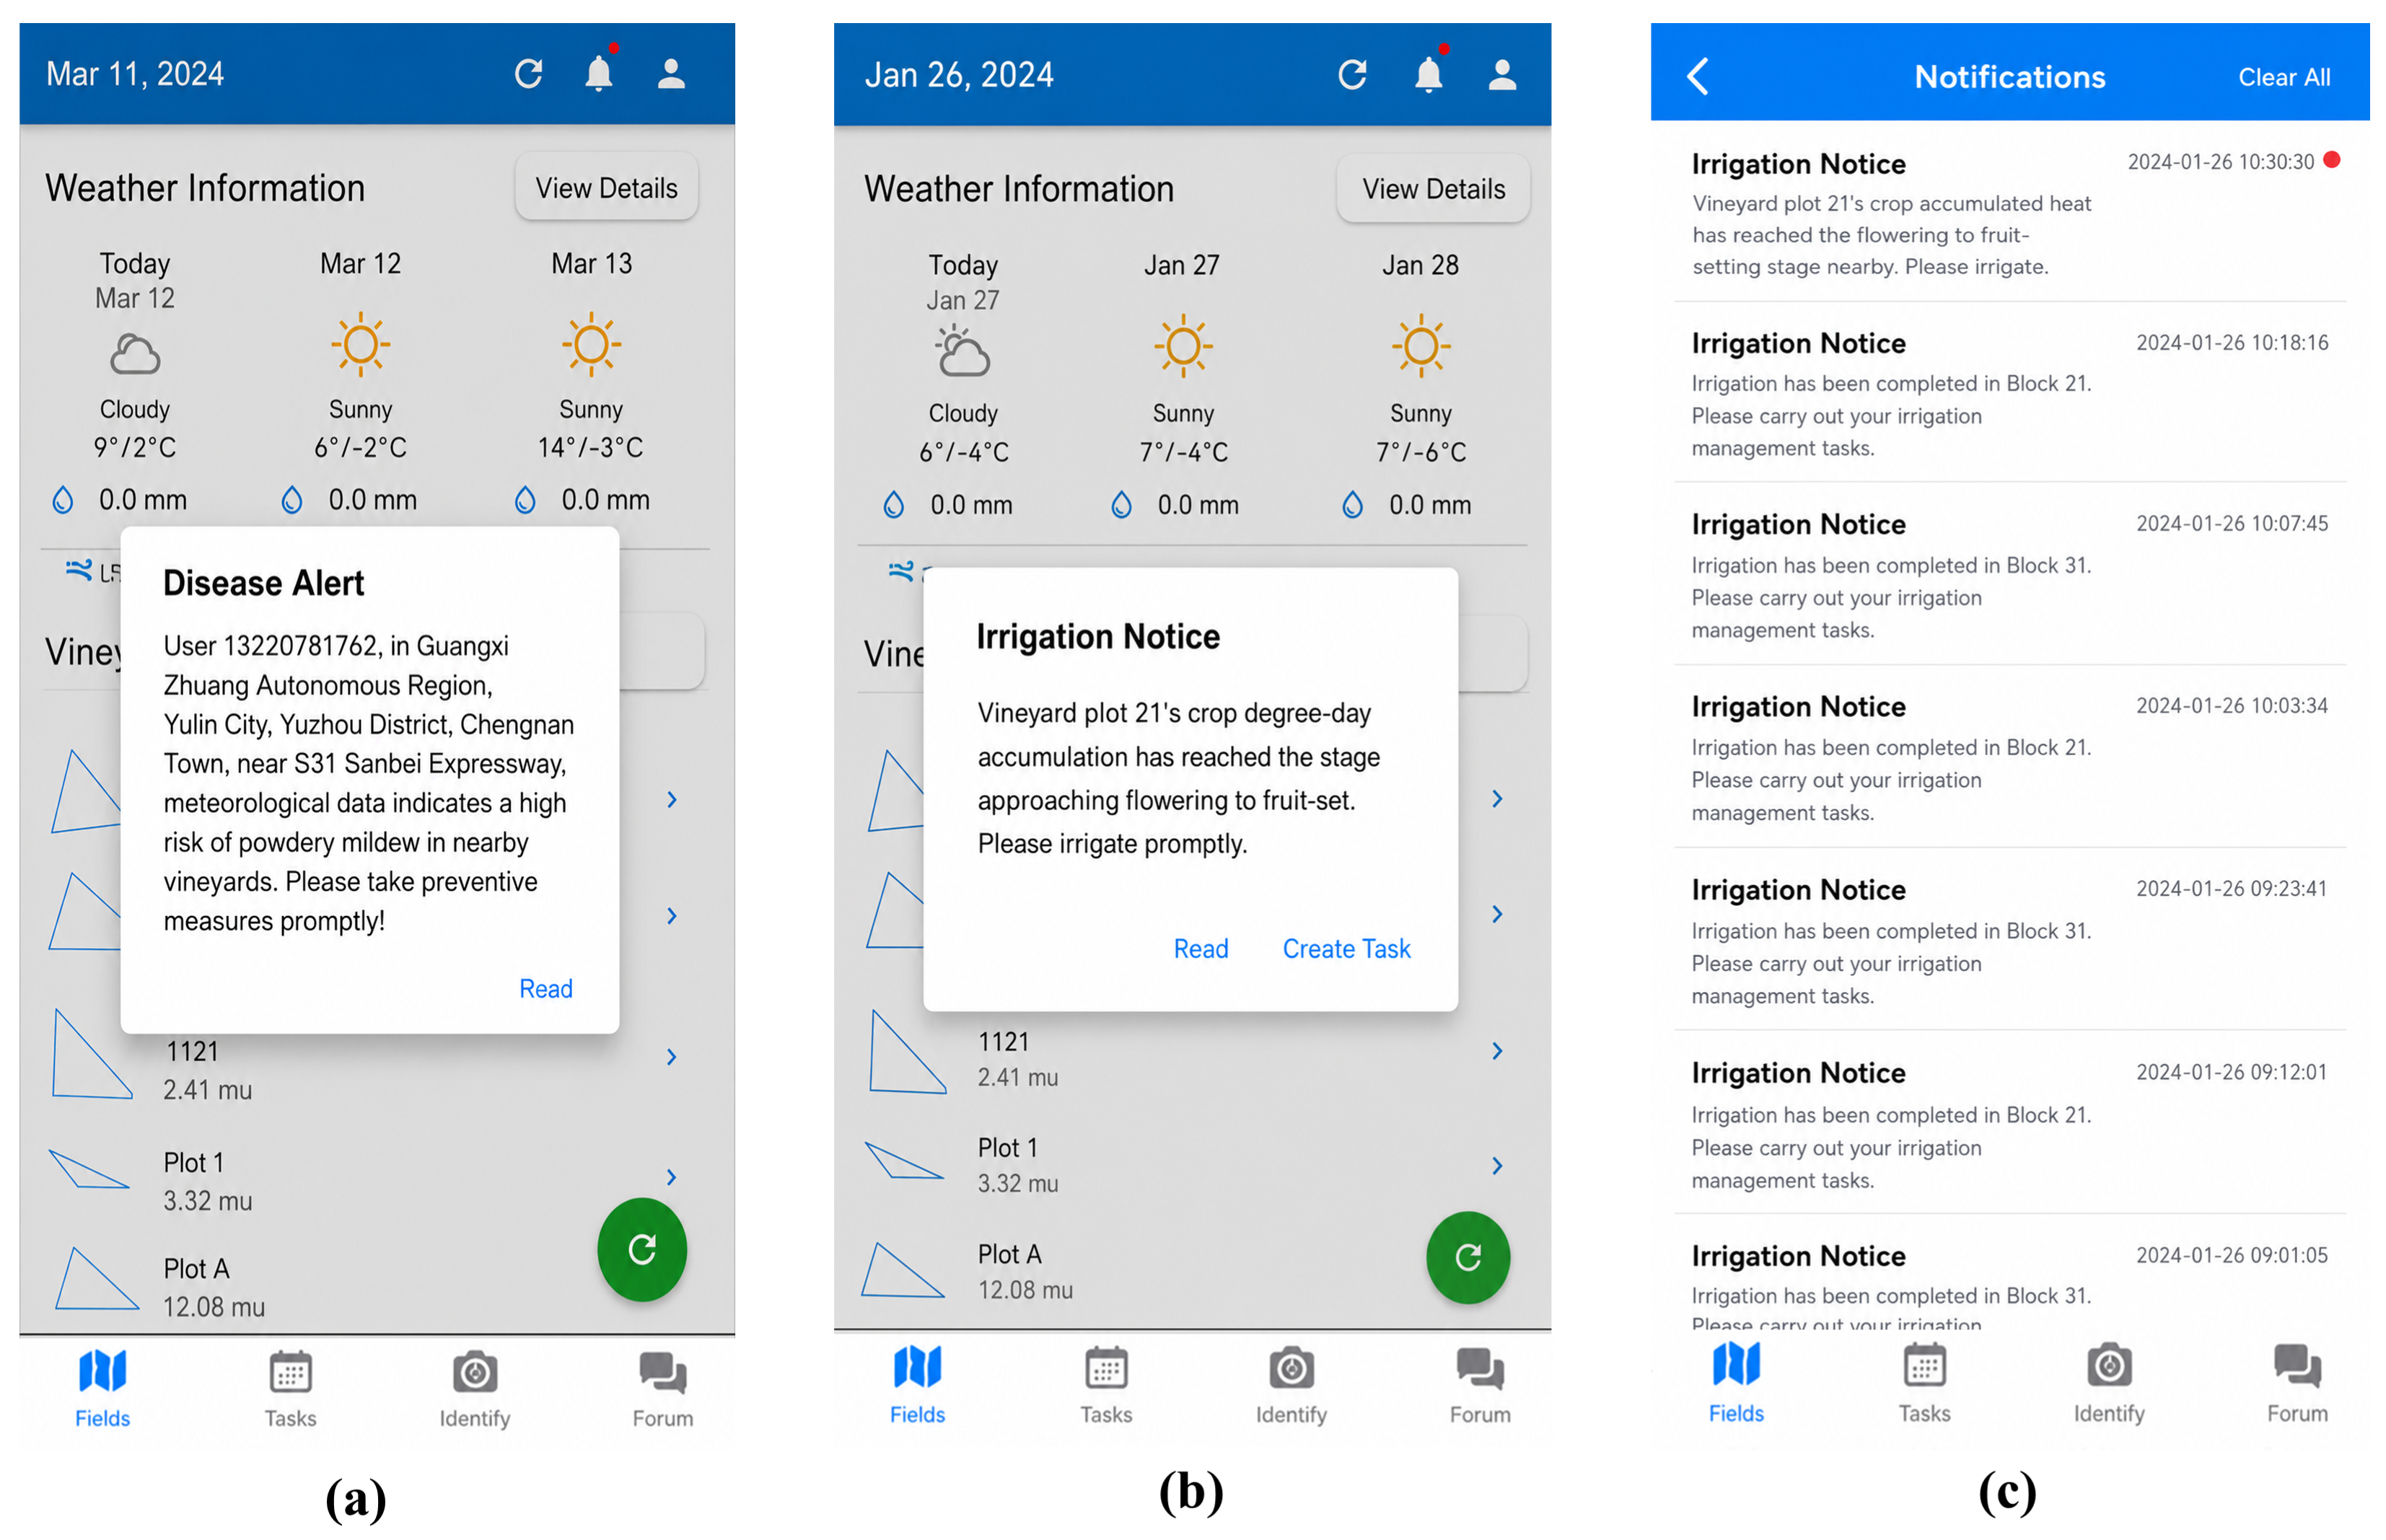
\includegraphics[width=\linewidth]{../fig/alert_notification_interfaces.png}
\caption[Alert and notification evidence for crop-season events]{Alert and notification evidence for crop-season events in GrapeMaster. (a) The disease-alert dialog displays a crop-season disease-risk event. (b) The management notice dialog provides a task-related prompt. (c) The notification list archives reviewable crop-season events.}
\label{fig:alert_notification_interfaces_result}
\end{figure}

\begin{figure}[H]
\centering
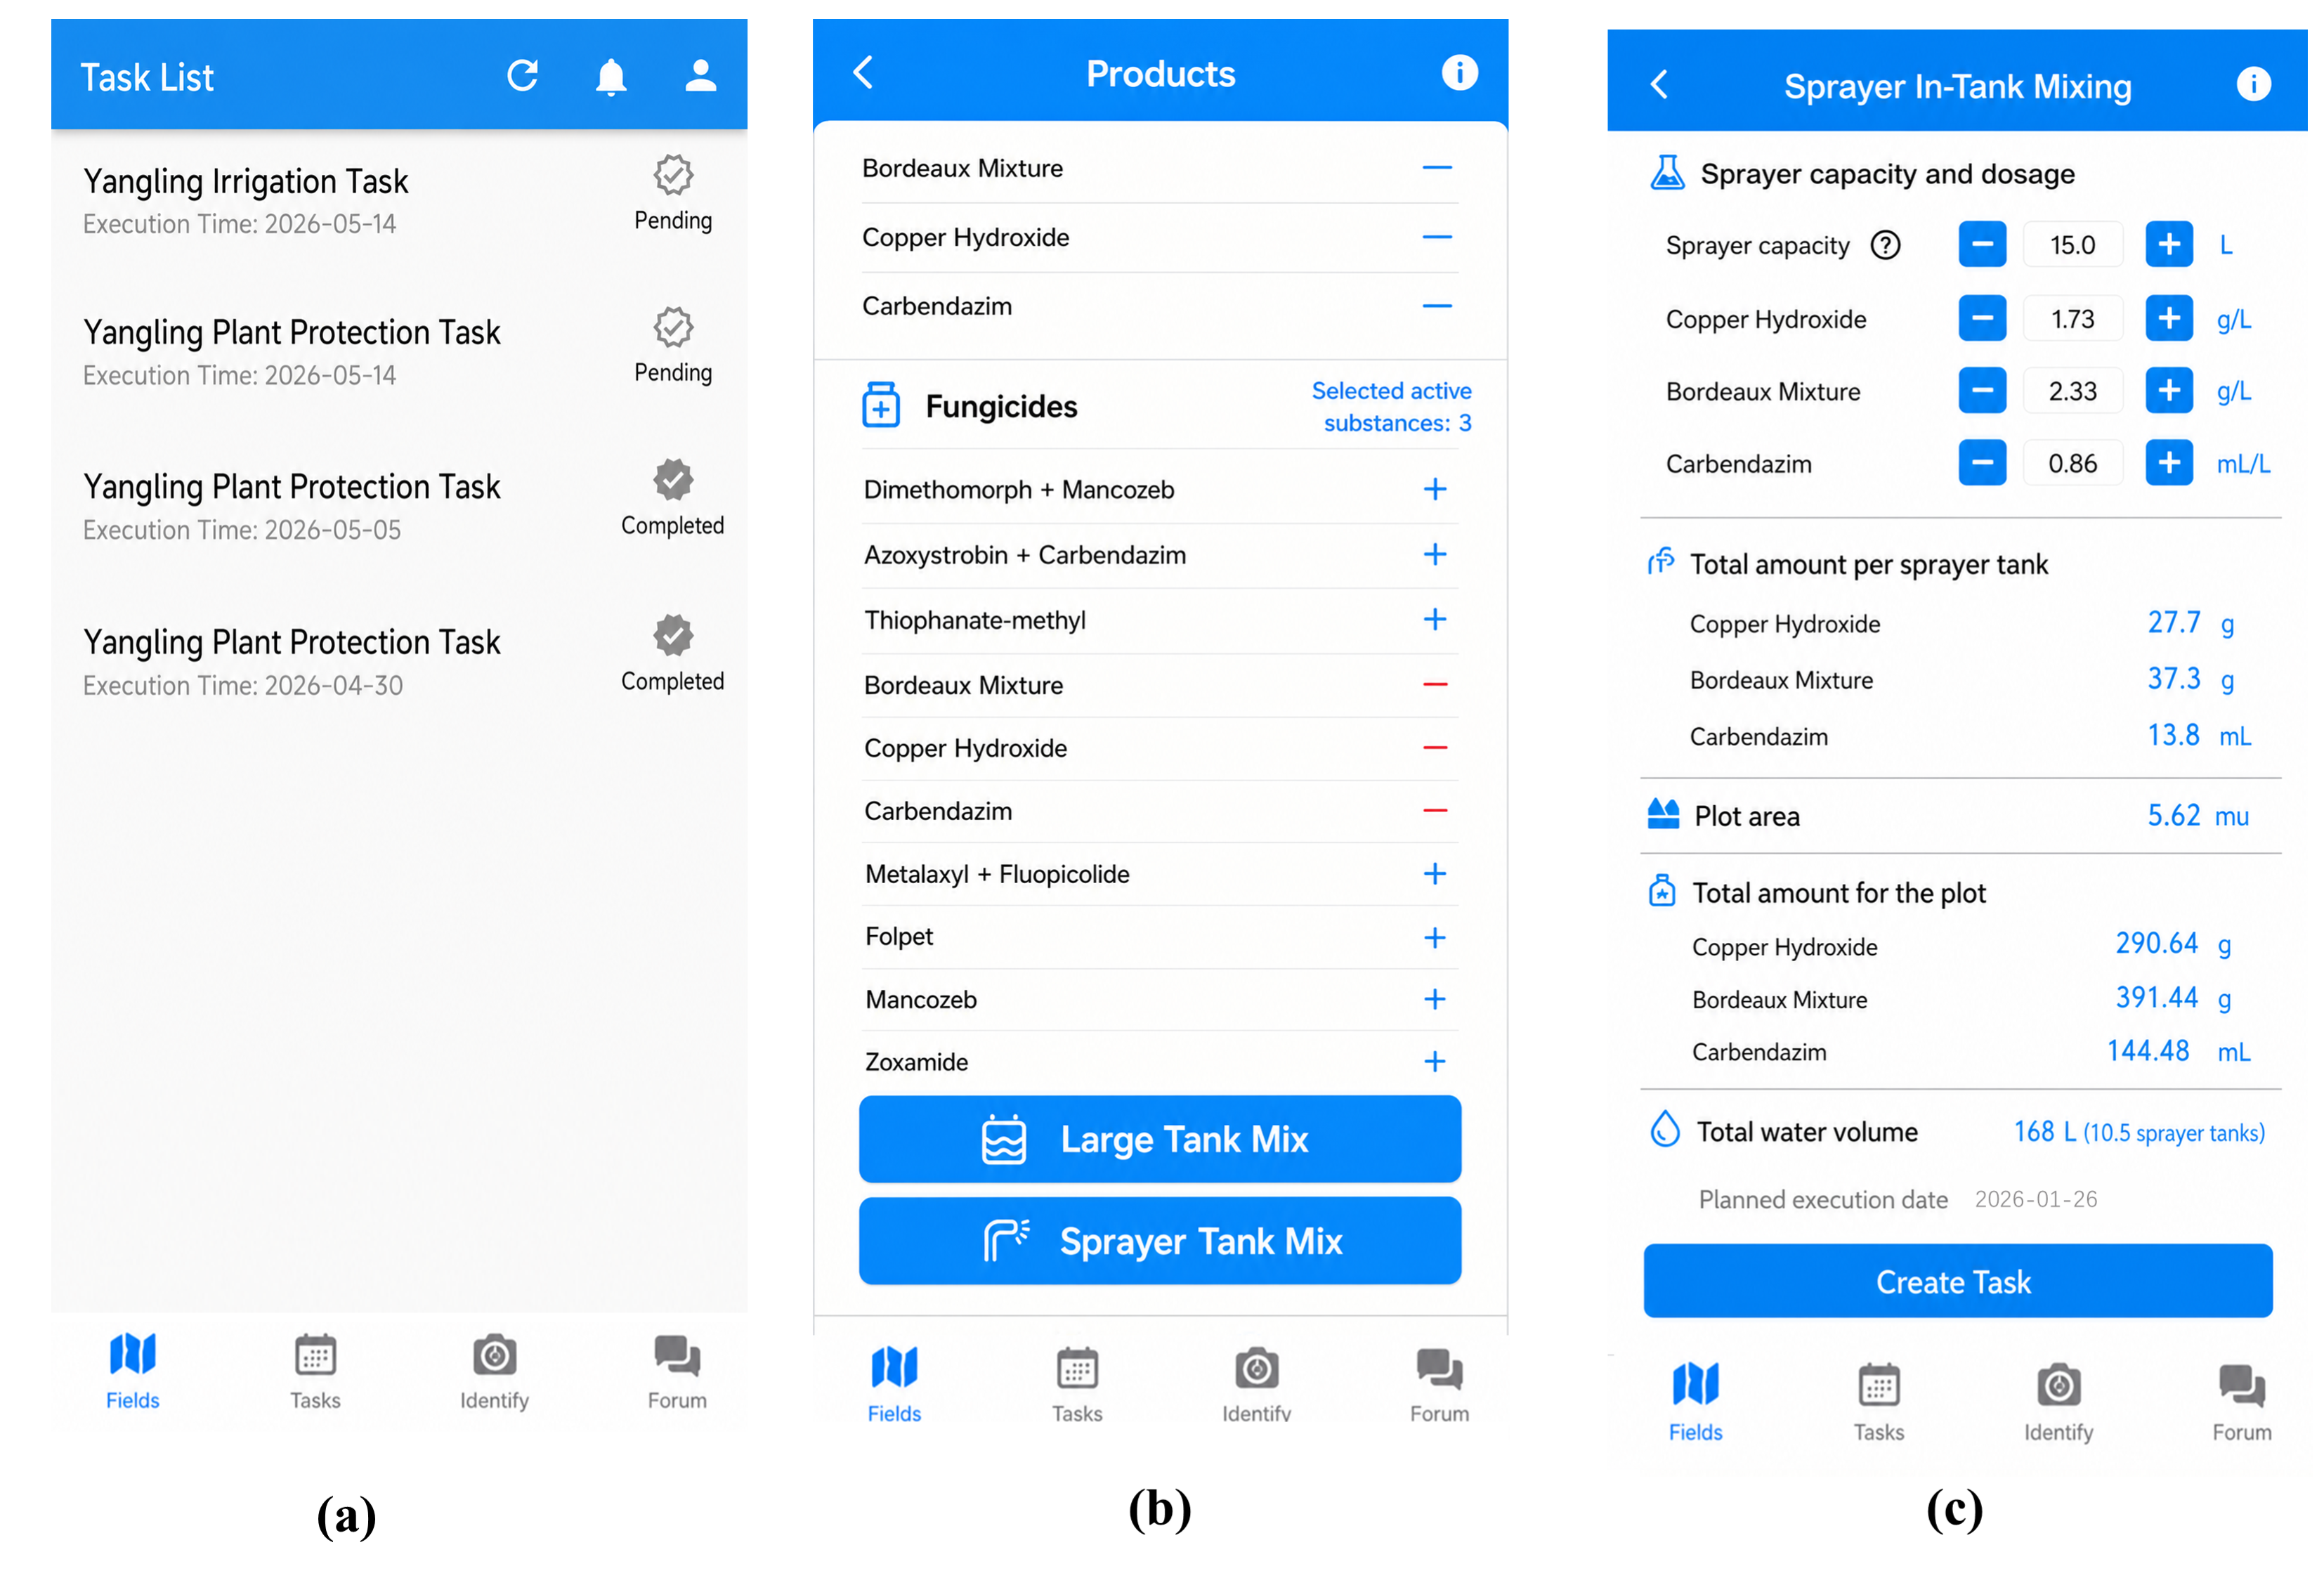
\includegraphics[width=\linewidth]{../fig/task_management_interfaces.png}
\caption[Task and product-feedback interfaces in GrapeMaster]{Task and product-feedback interfaces in GrapeMaster. (a) The task list records field operations and task status. (b) The product-selection page stores fungicide or pesticide entries linked to plant-protection tasks. (c) The in-tank mixing page records sprayer capacity, product dosage, plot area, water volume, and planned date.}
\label{fig:task_management_interfaces_result}
\end{figure}

\begin{figure}[H]
\centering
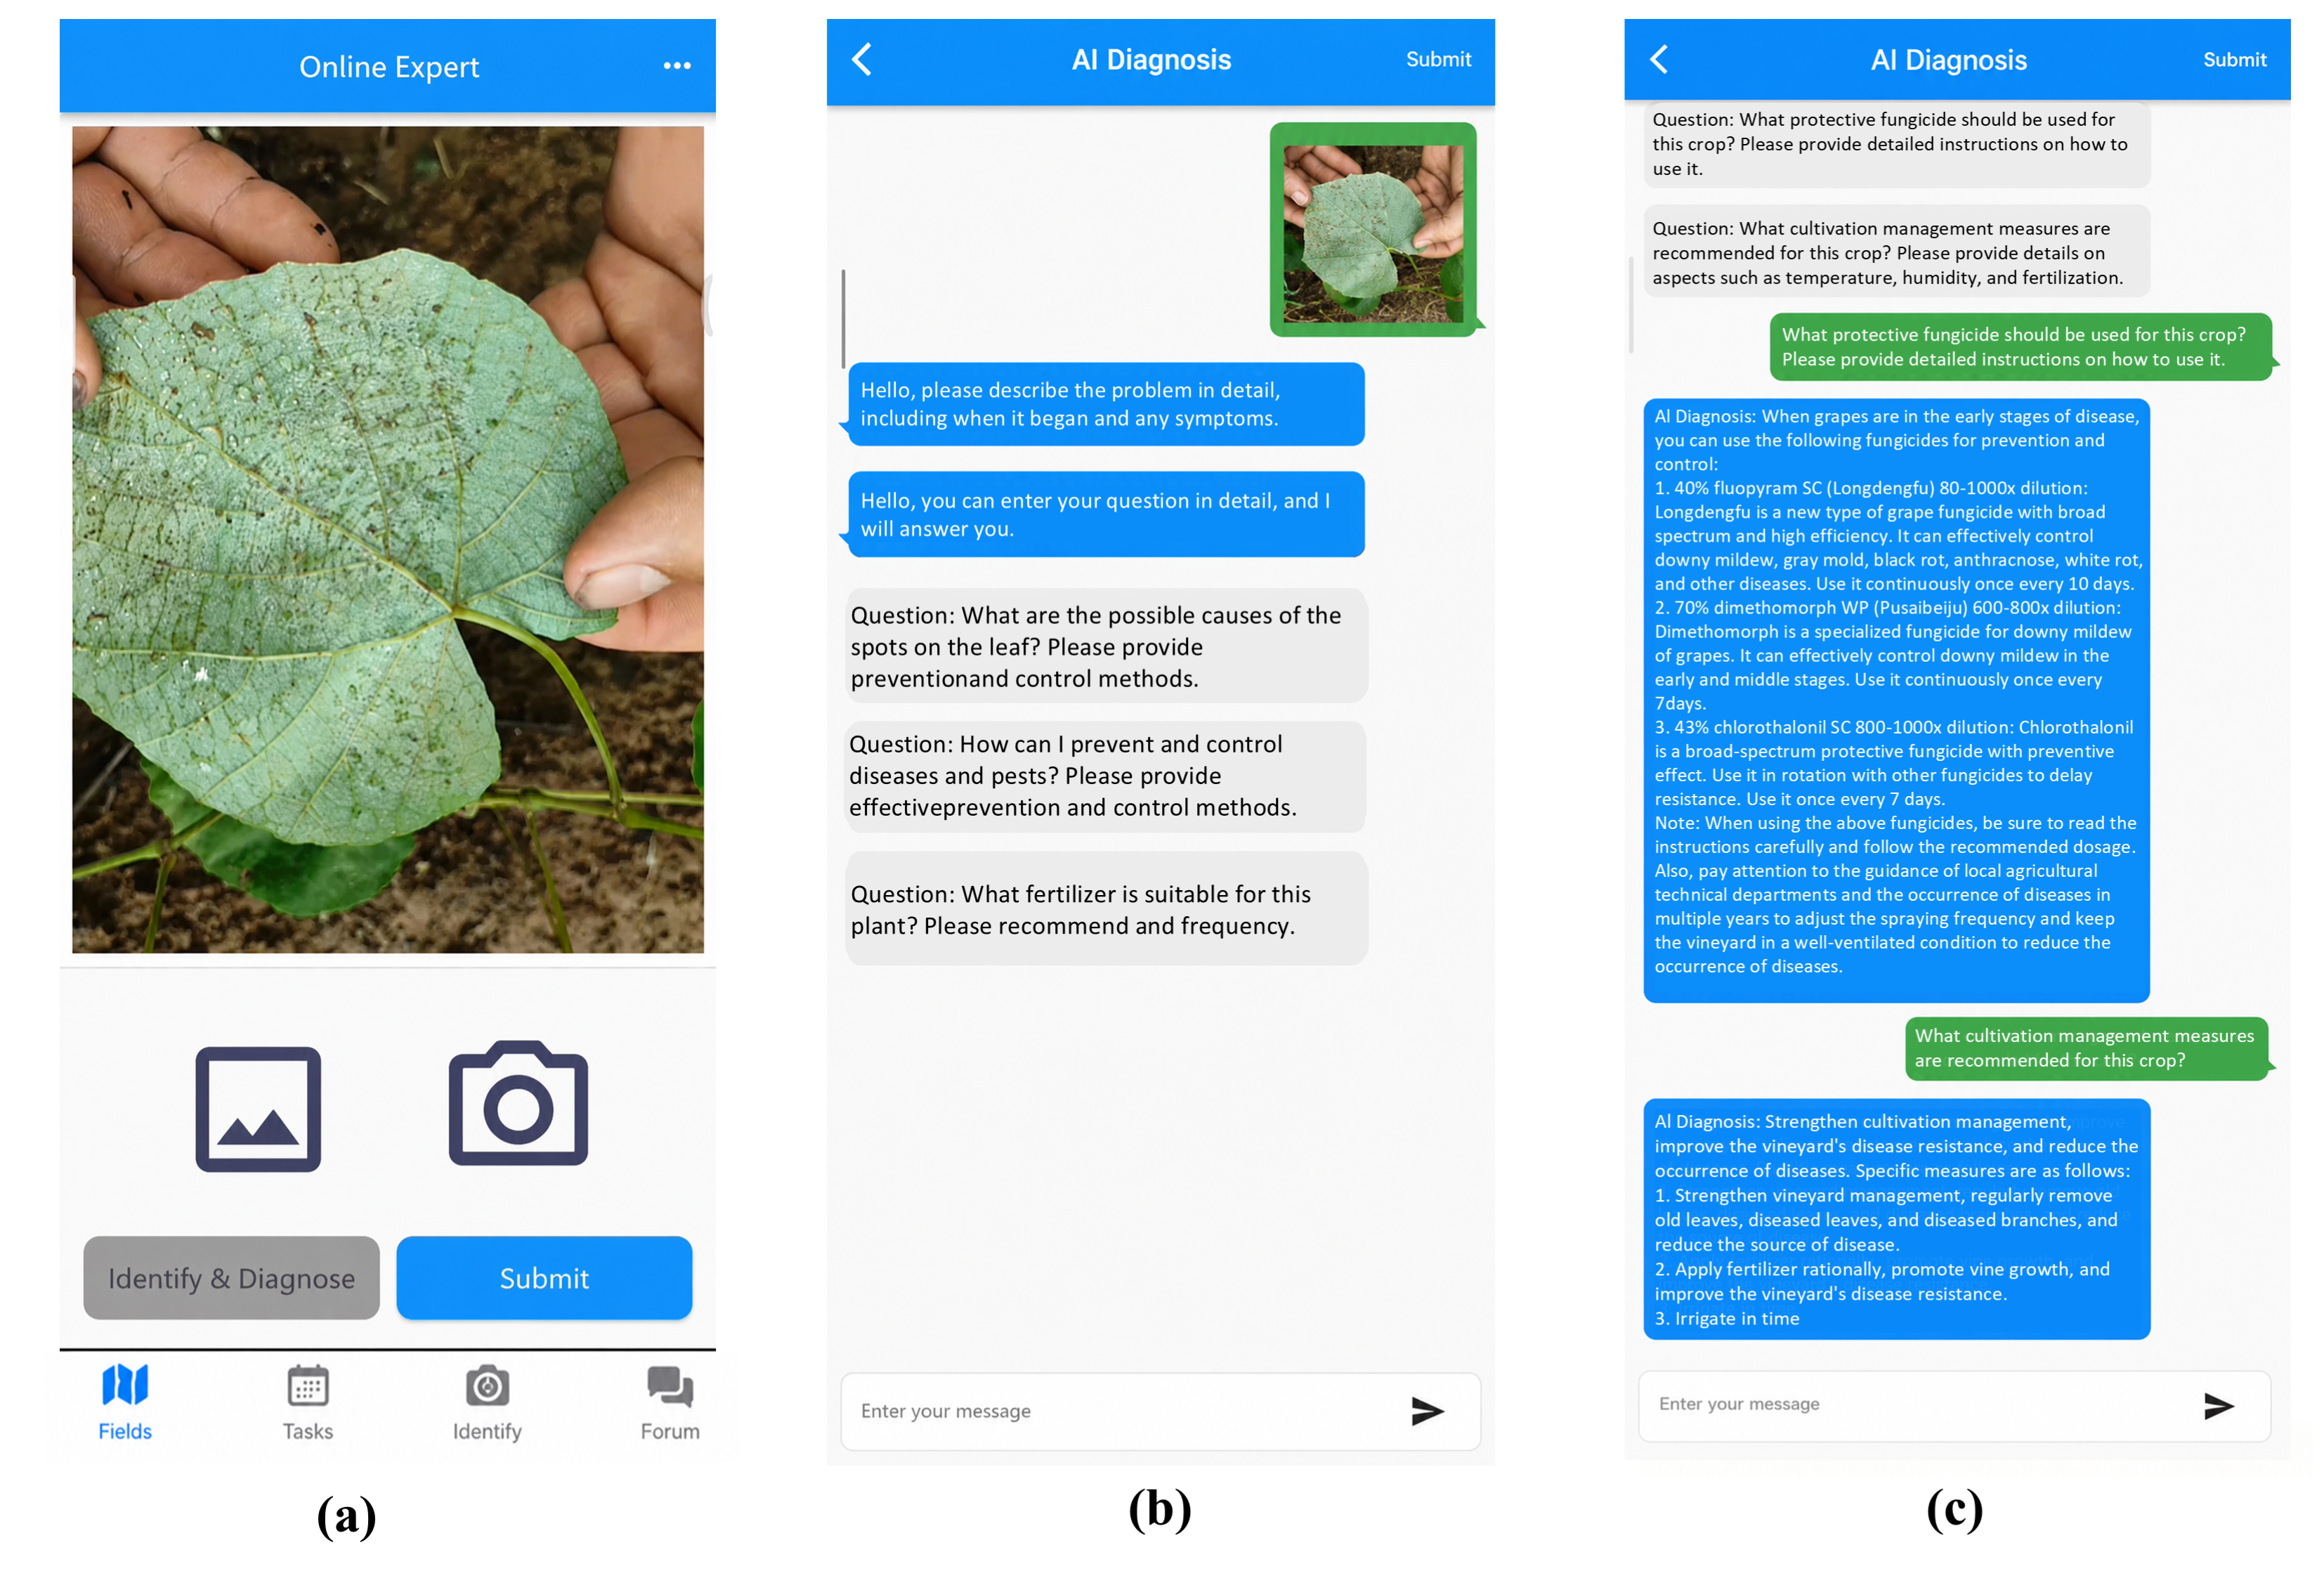
\includegraphics[width=\linewidth]{../fig/ai_diagnosis_interfaces.png}
\caption[Symptom-image and advisory evidence interfaces]{Symptom-image and advisory evidence interfaces in GrapeMaster. (a) The image-upload page records post-symptom visual evidence. (b) The recognition-result page displays the predicted grape disease category. (c) The advisory interface stores consultation text linked to the crop-season workspace.}
\label{fig:ai_diagnosis_interfaces_result}
\end{figure}

\subsection{Representative replay of the risk-to-feedback chain}\label{representative-crop-season-replay-of-the-closed-loop}

The selected chain-complete crop-season replay contained one weather payload, one phenology payload, one disease-risk payload, 53 notification records, two completed plant-protection tasks, and four fungicide-product records under the same crop-season UUID or linked task identifiers (Figure~\ref{fig:crop_season_replay_loop}; Table~\ref{tab:crop_season_replay_audit}). Figure~\ref{fig:crop_season_replay_loop} summarizes the retained record sequence from the crop-season management unit to state updating, risk interpretation, event delivery, task execution, and treatment feedback. Table~\ref{tab:crop_season_replay_audit} reports the corresponding records and identifiers.

No field-note or disease-incidence note was present under this replay anchor, although symptom-evidence records were present in the broader retained account set.

In this replay, weather, phenology, and disease-risk payloads shared the crop-season key; notifications and completed tasks were recorded under the same crop-season context; and fungicide-product records carried task identifiers. The absence of a field-note or incidence-note record was retained as an explicit missing-evidence entry.

\begin{figure}[H]
\centering
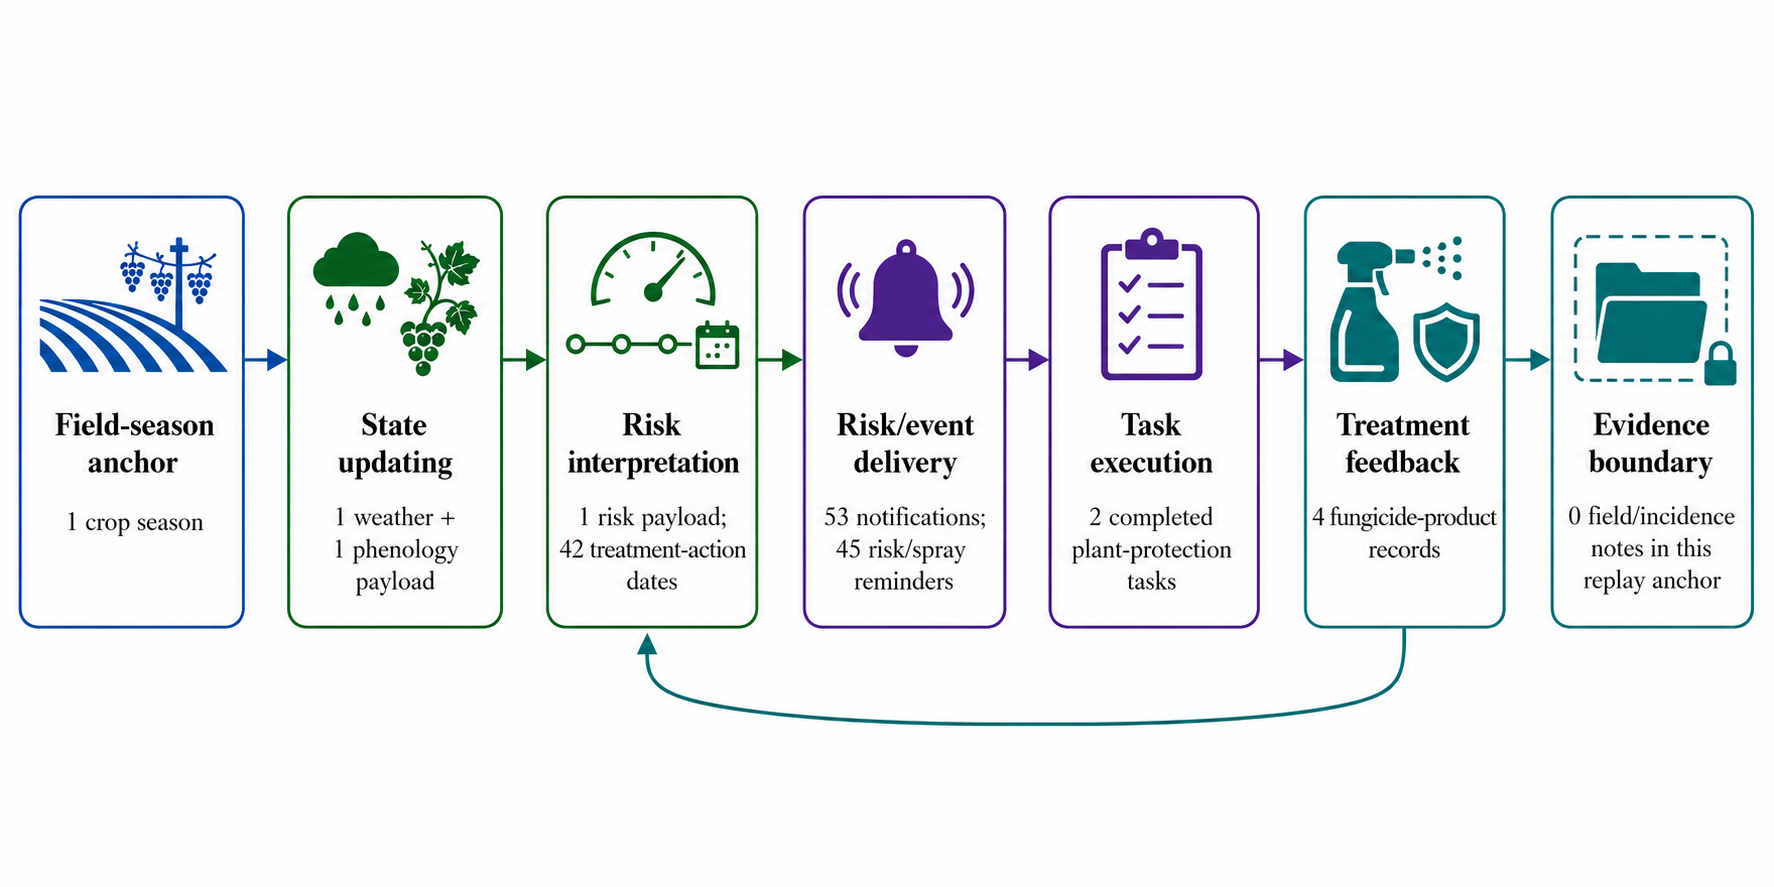
\includegraphics[width=\linewidth]{../fig/disease_feedback_loop.png}
\caption[Record-level replay of the risk-to-feedback chain]{Record-level replay of the risk-to-feedback chain in GrapeMaster. Each node summarizes retained records under the selected crop-season management unit. The absence node records the lack of field-note or incidence-note records for this replay case.}
\label{fig:crop_season_replay_loop}
\end{figure}

\begin{table}[H]
\centering
\begingroup
\setlength{\tabcolsep}{3pt}
\renewcommand{\arraystretch}{1.12}
\scriptsize
\caption{Record-level evidence in a representative crop-season replay in GrapeMaster.}
\label{tab:crop_season_replay_audit}
\begin{tabular}{p{0.20\linewidth} p{0.29\linewidth} p{0.19\linewidth} p{0.22\linewidth}}
\toprule
Record group & Record evidence & Identifier or status & Result note \\
\midrule
Replay record set & Weather, phenology, risk, notification, task, and fungicide records & One crop-season UUID & Representative crop-season replay \\
State and risk records & Weather, phenology, and disease-risk payloads & Shared crop-season key & Shared seasonal record set \\
Operation records & Notifications and completed plant-protection tasks & Same crop-season context & Notification and task records \\
Treatment-feedback records & Fungicide-product records & Task identifiers & Product-task record set \\
Missing-evidence entry & No field-note or incidence-note record & Explicit absence & No symptom note in this replay \\
\bottomrule
\end{tabular}
\endgroup
\end{table}

\subsection{Platform-compatible analytical module evidence}\label{trustworthy-analytical-modules-embedded-in-grapemaster}

The module-level result set included downy mildew first-infection timing, field-observed grapevine growth stages, and grape disease image-recognition metrics.

The FSIM-S configuration evaluated for GrapeMaster produced a validation mean absolute error of 6.3 days and a validation root mean square error of 6.5 days for downy mildew first-infection timing (Figure~\ref{fig:core_analytical_support_result}). The image-recognition module produced class-wise F1-scores from 0.926 to 0.998 across seven grape disease categories. Downy mildew, the disease target linked to FSIM-S risk prediction, reached an F1-score of 0.986.

The phenology dataset contained 151 valid field observations from six Guangxi site-years. In grouped three-fold validation, the broad-stage configuration reached 58.0\% exact major-stage agreement and 76.0\% user-visible agreement after transition-window display, with a mean absolute stage distance of 0.45 major stages when the sparsely observed post-harvest class was excluded from the core metrics. In Figure~\ref{fig:phenology_major_stage_validation_result}, most non-exact cases were transition-window or adjacent-stage cases, and severe mismatches represented a small fraction of observations. Fruit development and ripening stages had lower mean stage distance than early-season stages. The wk cultivar subset contained one sparse site-year and is shown separately from the two larger cultivar subsets.

\begin{figure}[H]
\centering
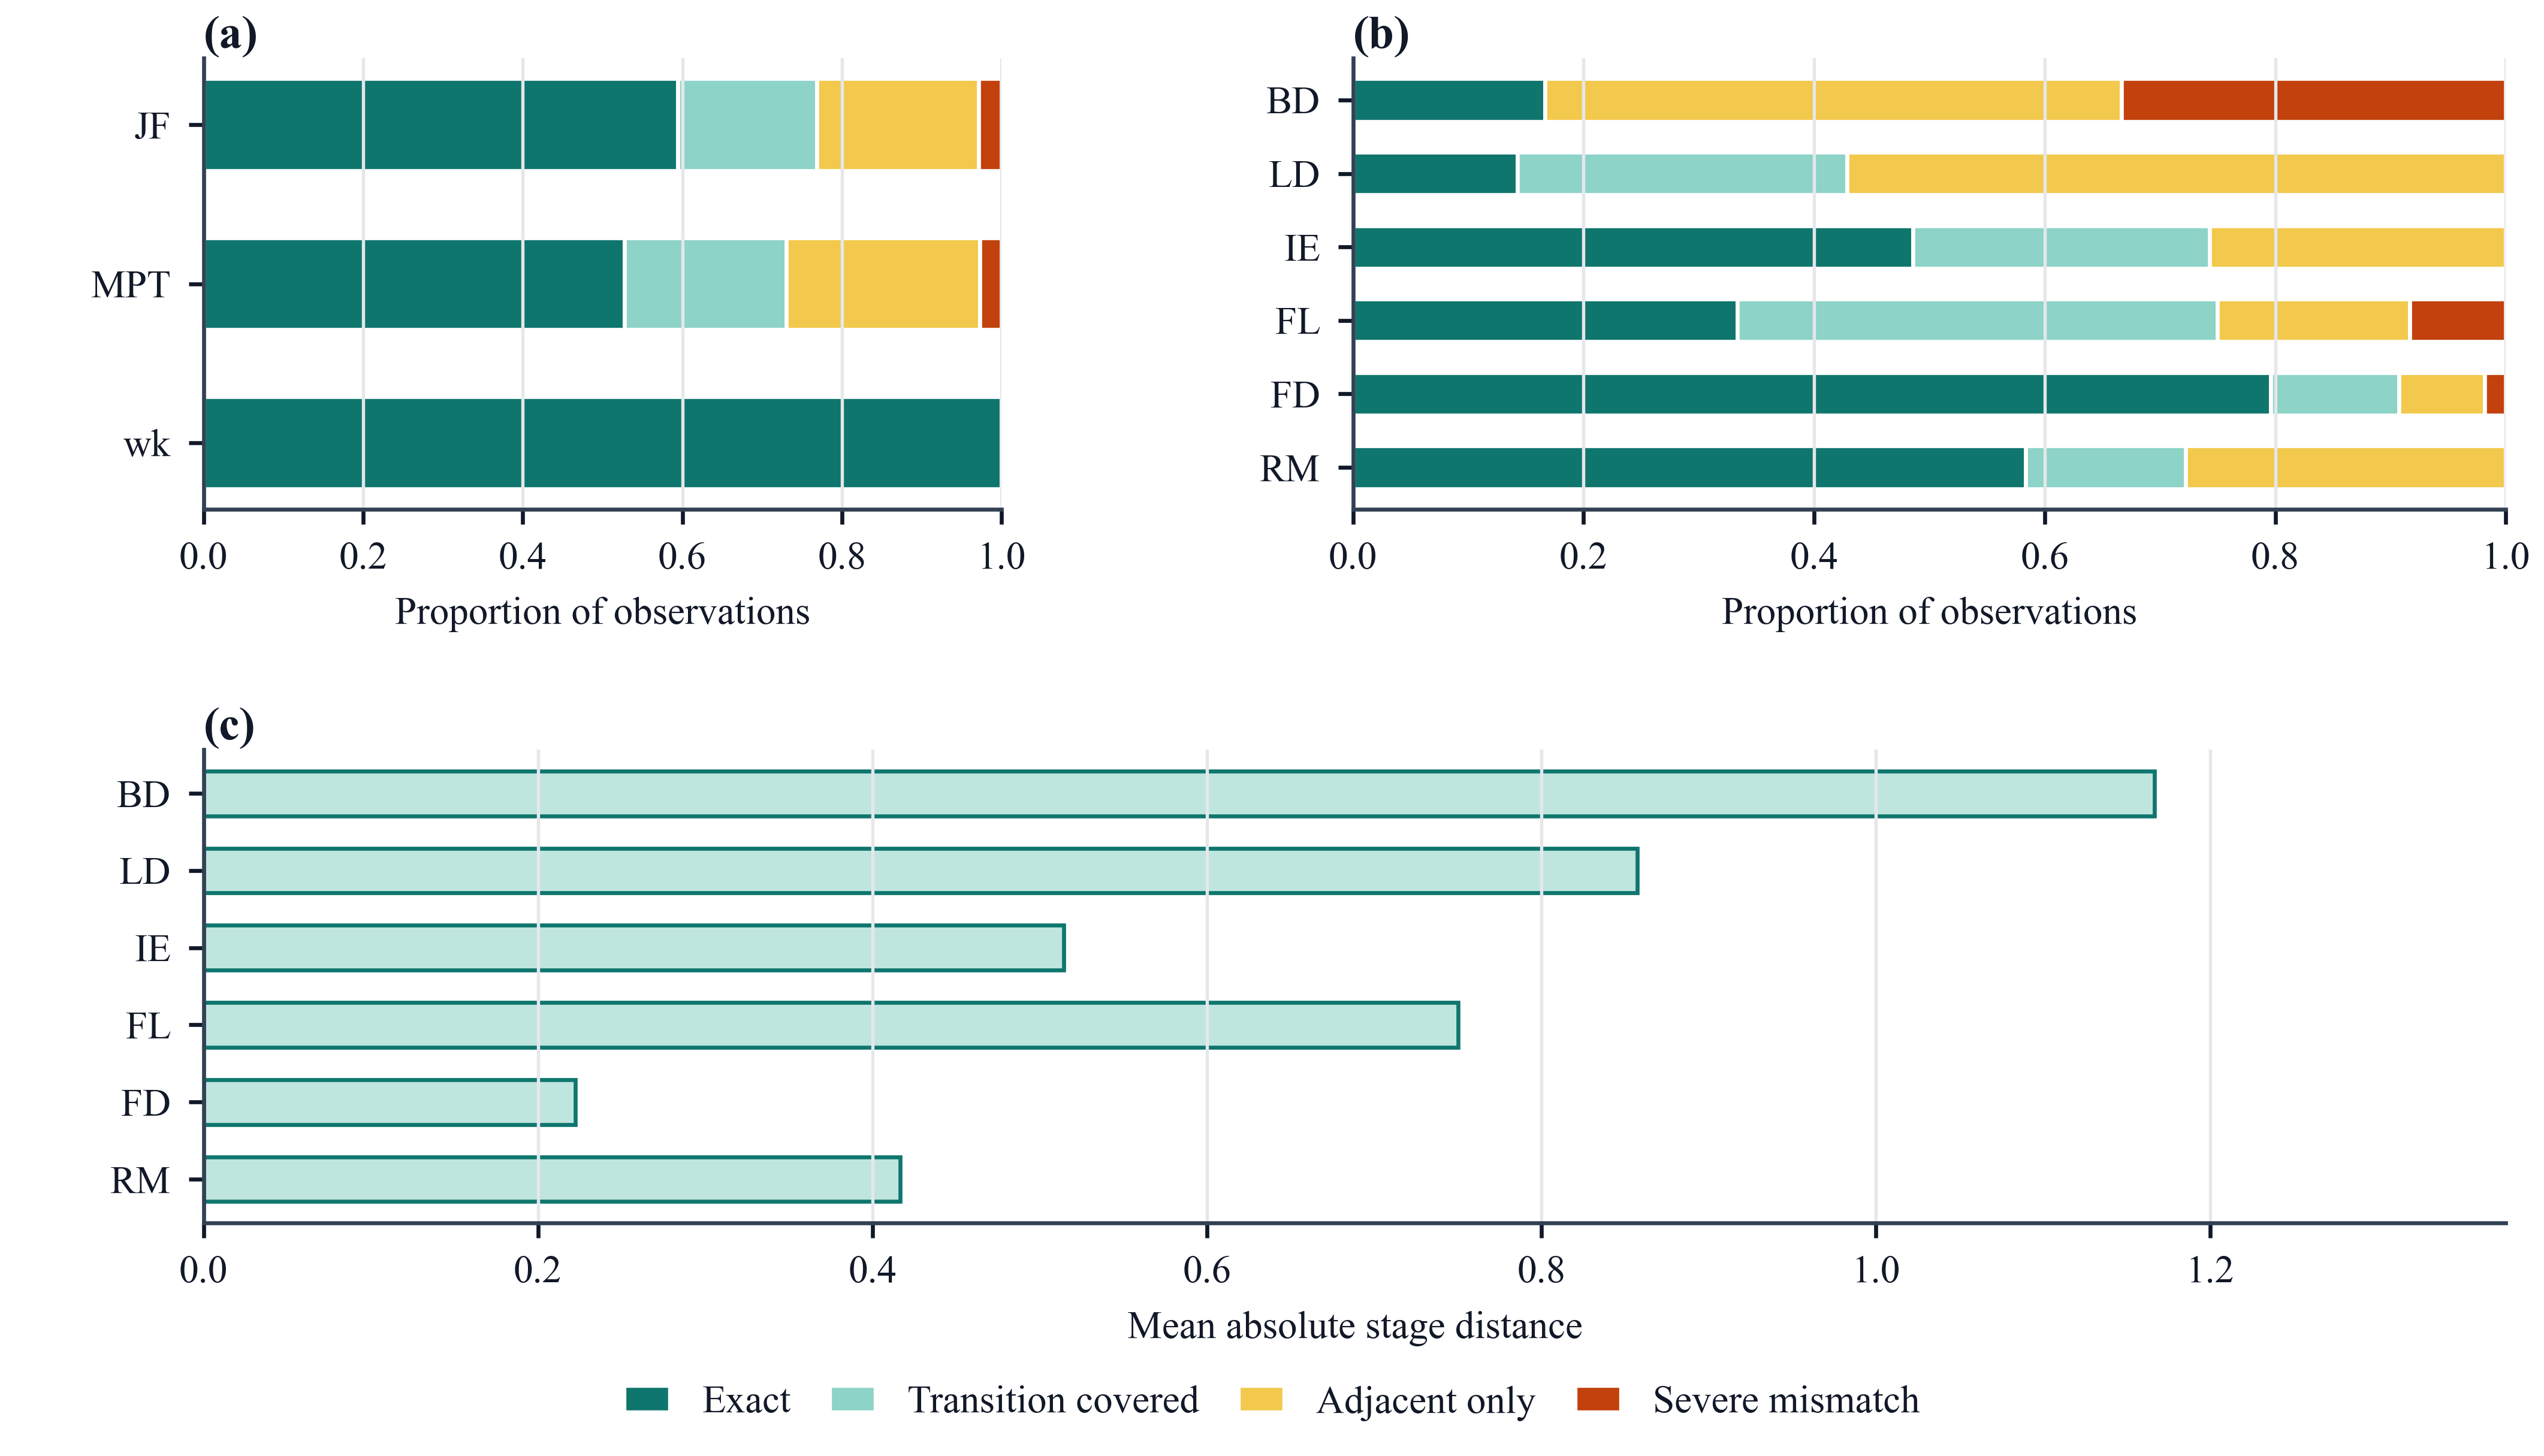
\includegraphics[width=\linewidth]{../fig/phenology_major_stage_validation.png}
\caption[Validation evidence for the broad-stage phenology module]{Validation evidence for the platform-compatible broad-stage phenology module. (a) Outcome proportions are summarized by cultivar. (b) Outcome proportions are summarized by observed major stage. (c) Mean absolute stage distance is summarized by observed major stage. BD, bud development; LD, leaf development; IE, inflorescence emergence; FL, flowering; FD, fruit development; RM, ripening of berries.}
\label{fig:phenology_major_stage_validation_result}
\end{figure}

\begin{figure}[H]
\centering
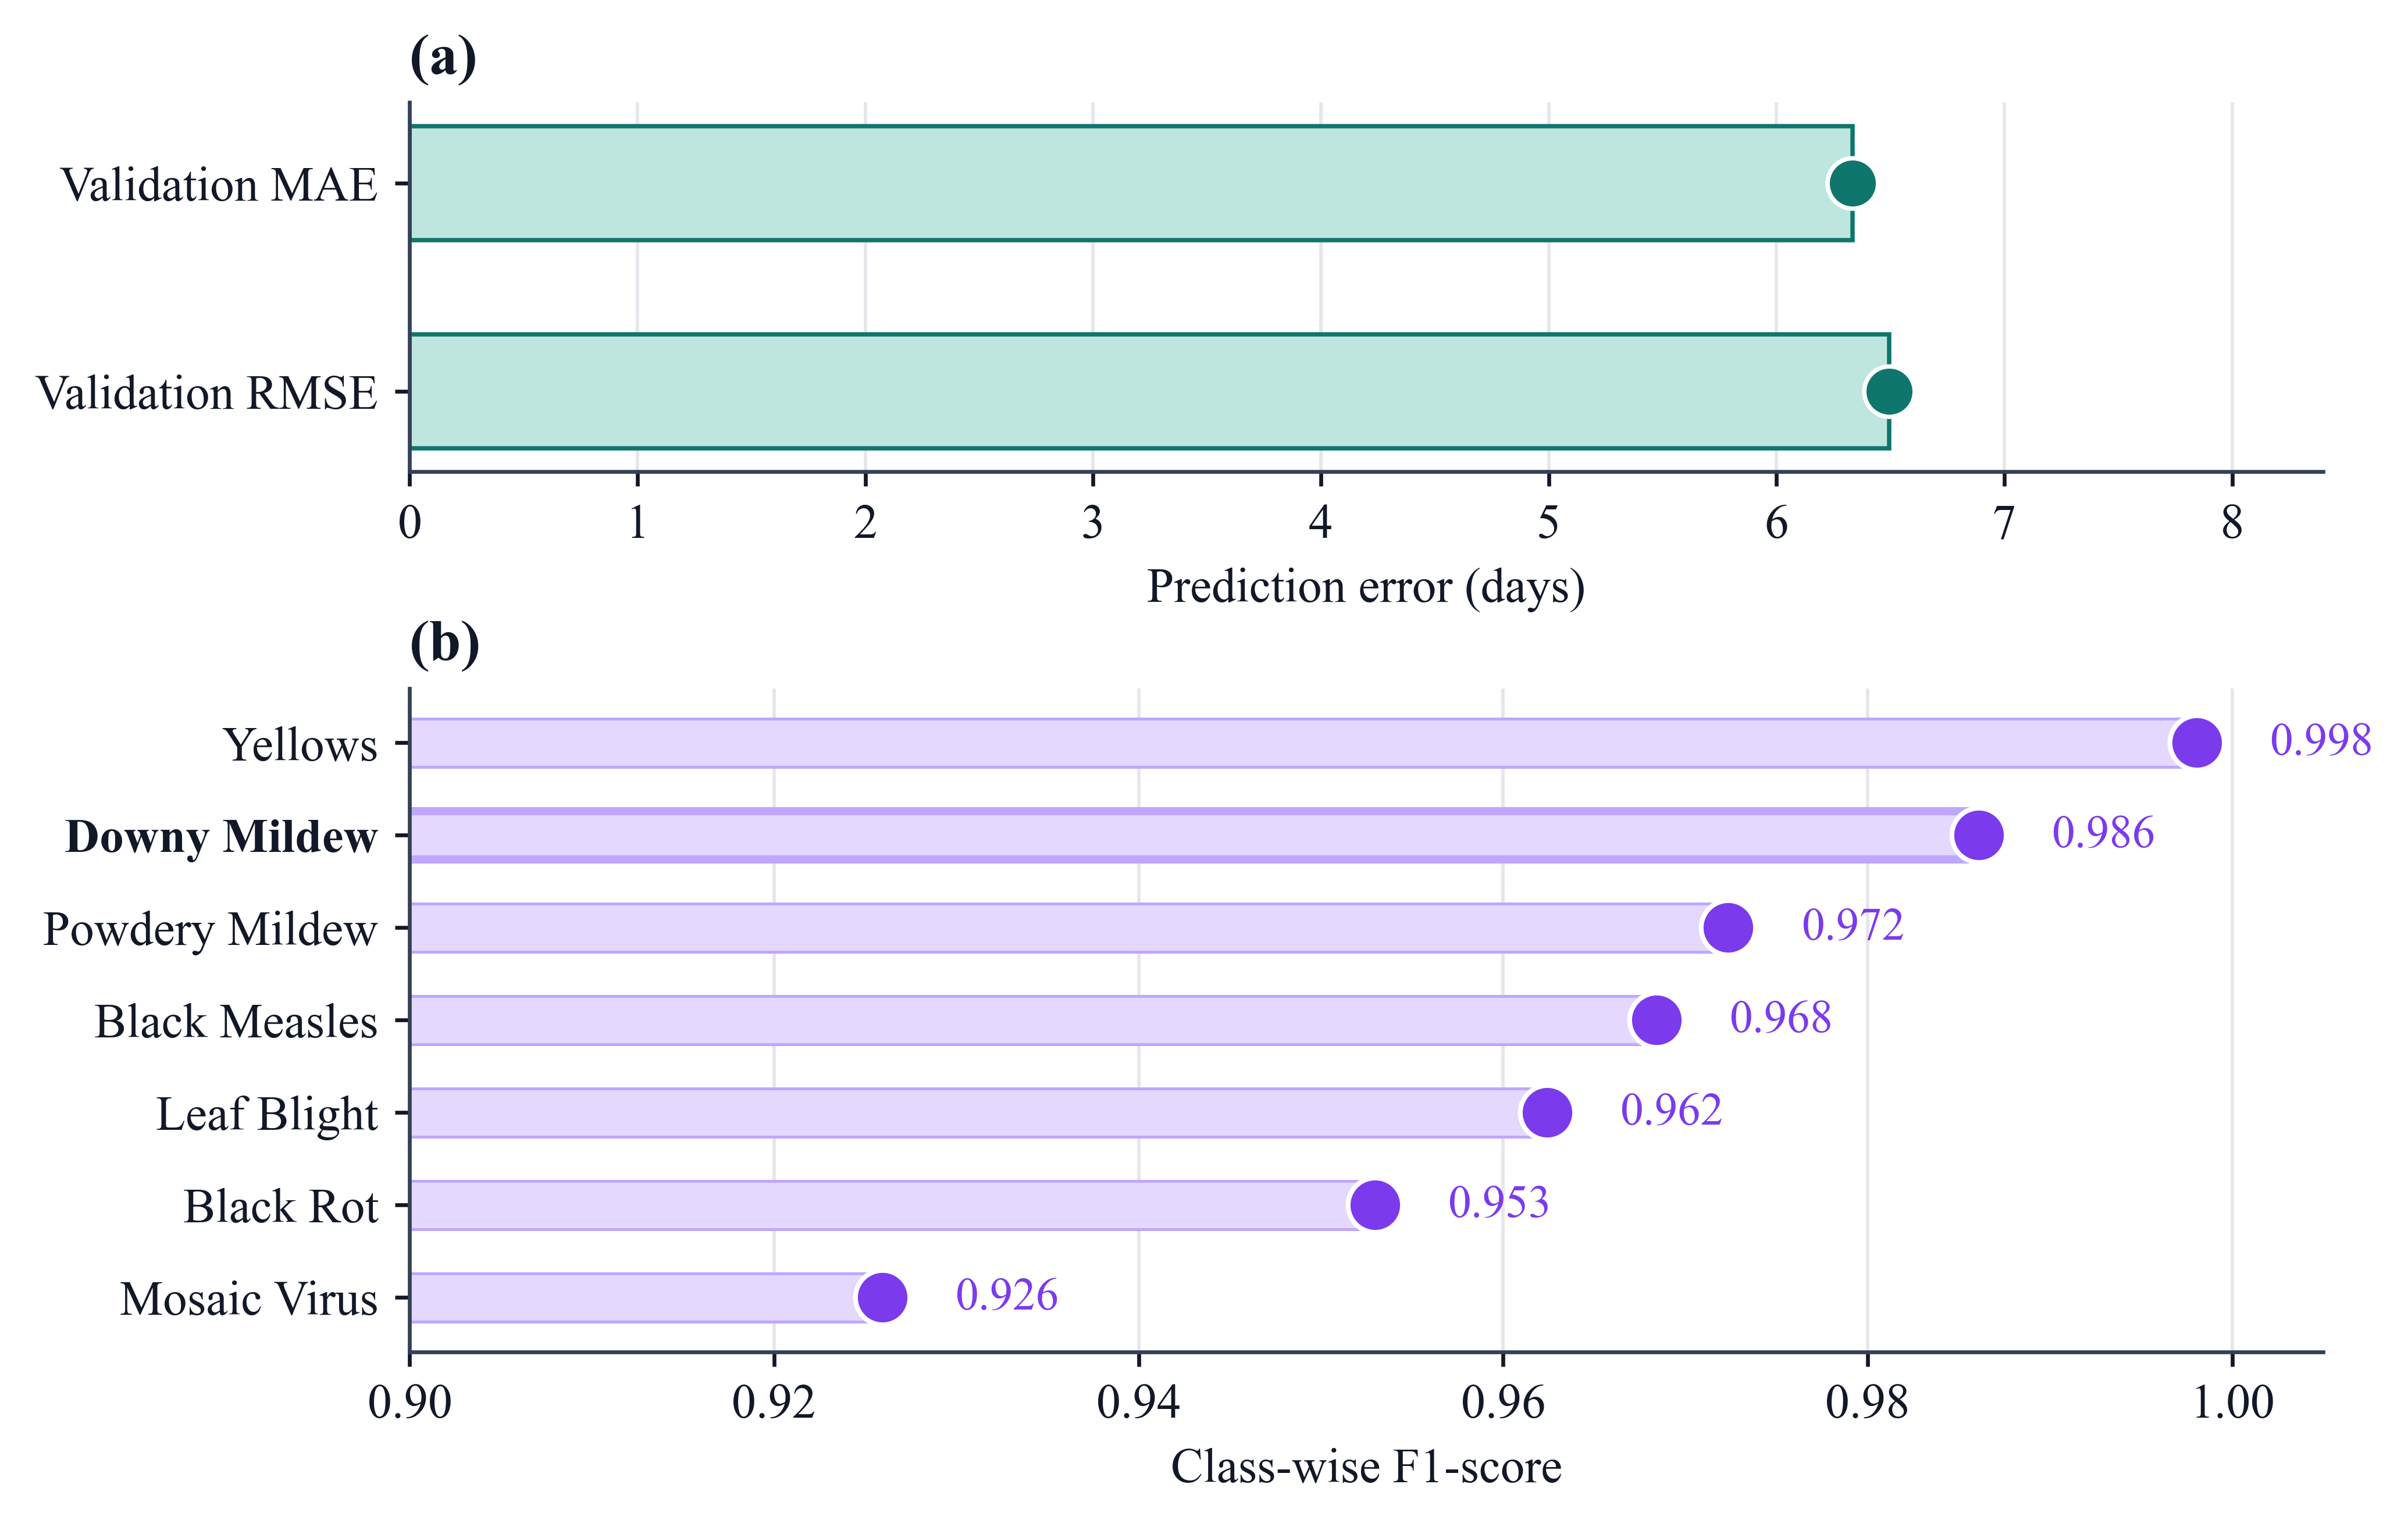
\includegraphics[width=\linewidth]{../fig/fsims_supporting_performance.png}
\caption[Module-level evidence for disease-risk and image-recognition components]{Module-level evidence for disease-risk and image-recognition components. (a) The FSIM-S panel reports validation error for downy mildew first-infection timing. (b) The image-recognition panel reports class-wise F1-scores for grape disease categories, with downy mildew highlighted.}
\label{fig:core_analytical_support_result}
\end{figure}

\section{Discussion}\label{discussion}

\subsection{Crop season as the platform integration unit}\label{crop-season-records-as-the-integration-unit}

In GrapeMaster, the crop season is used as the platform-level management unit for organizing vineyard disease-management workflows, not merely as an agronomic time label or database field. Vineyard disease management is not organized around a single observation or model output; it develops across the production season as weather exposure, crop-stage change, disease-risk interpretation, field operation, treatment feedback, symptom evidence, and season review are successively generated and updated. At the data and workflow level, this management unit is implemented as a traceability object that links field configuration, weather, phenology, disease risk, notifications and tasks, fungicide or pesticide feedback, symptom images, advisory interaction, and archived records. The design contribution is that the platform architecture matches the temporal structure of grape disease management: the field remains geographically stable, whereas weather exposure, phenological stage, inoculum pressure, protection status, observations, and decisions are redefined within each production season. This need for a season-specific management unit is consistent with previous plant disease DSS studies showing that weather-driven models and advisory systems improve decision timing only when their outputs are usable within operational contexts \citep{seemForecastingPlantDisease2004,rossiAddressingImplementationProblem2014,bregaglioPublicDecisionSupport2022}. It is also consistent with grapevine phenology studies showing that cultivar and regional climatic context condition crop-stage interpretation, making seasonal anchoring necessary for operational disease management rather than merely convenient for data storage \citep{parkerGeneralPhenologicalModel2011,wangAssessingGrapevinePhenological2020}.

This crop-season-centered architecture has three operational consequences. Cross-module retrieval can be performed through a shared seasonal management unit rather than by manually reconstructing links among field, weather, risk, task, image, advisory, and record tables. Season replay becomes possible because risk states, notifications, completed tasks, treatment feedback, and later evidence can be reconstructed within a single temporal frame. Repeated seasons from the same field can also support longitudinal comparison using comparable seasonal histories rather than isolated records, which is especially relevant for perennial grapevine systems whose growth and disease consequences extend within and across years \citep{nogueirajuniorModellingDynamicsGrapevine2018b}. These functions distinguish a crop-season-centered platform from field- or user-centered record systems in which season remains a descriptive attribute rather than the management unit that links prediction, action, feedback, evidence, and review.

The architecture-level linkage evidence is relevant because the retained records remained interpretable through this shared management unit, not because of record volume alone. In this sense, the crop-season record is the data-level implementation of a broader platform integration strategy: it keeps analytical payloads, event delivery, field operations, treatment feedback, evidence objects, and archives retrievable within the same temporal and relational frame. The system-level contribution is therefore a traceability architecture that connects analytical outputs with executable actions and replayable records through explicit workflow relationships, database links, and verification rules, rather than a new standalone disease, phenology, or image-recognition algorithm.

\subsection{Traceability from risk display to field-operation feedback}\label{traceability-from-risk-display-to-field-operation-feedback}

GrapeMaster converts a stand-alone disease-risk warning into a risk-task-protection-feedback process. A warning model can identify favourable infection windows, but a warning output alone does not show whether the information was reviewed, converted into a task, followed by treatment, or reflected in a subsequent protection state. Disease-warning studies similarly indicate that prediction value should be interpreted through action-relevant probability and decision context rather than through risk classification alone \citep{yuenBayesianAnalysisPlant2002,zhaoDatadrivenModelSimulating2011}.

The representative replay provides workflow-closure evidence for this continuity. Weather and phenology inputs were linked to risk display and notification, warning states were connected with plant-protection tasks, completed tasks generated fungicide-product records, and those records supported later protection-state interpretation. This replay demonstrates that a disease-risk signal can move beyond passive warning display and become an executable, feedback-enabled, and reviewable management sequence within the same crop-season context. It does not measure agronomic efficacy, pesticide reduction, or grower adoption, but it establishes the evidence chain required to evaluate those outcomes in later production studies.

The symptom-image and advisory records form a supplementary evidence branch within the same seasonal frame. They do not replace the risk-task-protection-feedback chain, but they allow observed symptoms, diagnostic outputs, consultation messages, and later field notes to be reviewed together with the risk and operation history when those records are present.

The feedback step is essential because field treatment changes the state to which later warnings apply. In grapevine downy mildew management, subsequent interpretation depends not only on infection favourability, but also on recent fungicide use, product behaviour, rainfall, host growth, and disease pressure \citep{caffiFungicideModelsAre2018,bleyerTogetherBetterImprovement2020,warnekeEffectFungicideMobility2020}. GrapeMaster therefore treats completed plant-protection tasks as management feedback that updates an interpretable protection state. This state logic matters because a favourable infection period after a completed fungicide task is not equivalent to the same risk period without treatment feedback. Such traceability is a prerequisite for evaluating treatment timing, unnecessary fungicide use, and disease-control outcomes, particularly because fungicides remain a major pesticide class with environmental exposure concerns \citep{zubrodFungicidesOverlookedPesticide2019}.

\subsection{Deployment implications for vineyard digital disease management}\label{deployment-implications-for-vineyard-digital-disease-management}

Disease-risk models, phenology models, image-recognition models, and advisory models have become increasingly capable, but they are commonly developed, validated, and deployed as separate functions \citep{bregaglioPublicDecisionSupport2022,yanCDIPChatGLM3DualmodelApproach2025}. Farm-management platforms may place these functions in parallel menus or embed them as service modules, yet co-location does not by itself create a workflow that carries a risk signal into task execution, treatment feedback, symptom evidence, and season review. Disease-specific DSSs, including grapevine downy mildew warning models, can provide strong infection-risk outputs, but many stop at the warning or advisory layer \citep{orlandiniPLASMOSimulationModel1993,parkDMCASTPredictionModel1997,caffiEvaluationWarningSystem2010,caffiFungicideModelsAre2018}. General IoT and remote-sensing platforms connect heterogeneous data streams, but do not necessarily embed crop- and disease-specific logic for translating a risk signal into a vineyard operation \citep{bakirScalableEndtoendIoT2026,nkwochaEndtoendDigitalFramework2025}.

GrapeMaster is positioned at the intersection of these categories. It retains record-oriented farm-management functions, incorporates disease-risk, phenology, image, and advisory modules, and keeps their outputs interpretable within the same seasonal context. This combination is consistent with biovigilance frameworks that emphasize connecting observations, risk interpretation, and management decisions under changing production conditions \citep{carisseUsingBiovigilanceApproach2017}. Published systems rarely make the crop-season management unit, risk-task-protection-feedback logic, and grape disease-management modules explicit within a deployable platform for humid subtropical vineyards.

The same architecture also creates a practical route for regional extension. The current deployment uses routine field records and public weather data as a lightweight baseline, while allowing orchard-scale weather stations, phenology cameras, spore samplers, or other IoT sensors to be added when finer microclimate, crop-stage, or inoculum information is needed for field-scale management \citep{bakirScalableEndtoendIoT2026,nkwochaEndtoendDigitalFramework2025,brischettoCanSporeSampler2020,raiAdvancingSitespecificDisease2026}. In parallel, user-reported phenological stages, disease occurrence, treatment feedback, and field notes can serve as confirmatory evidence for correcting or contextualizing model and advisory outputs, a requirement emphasized in DSS implementation studies where local observations and advisory workflows shape operational use \citep{rossiAddressingImplementationProblem2014,seemForecastingPlantDisease2004,gonzalez-dominguezPlantDiseaseModels2023}. These two extension routes allow the platform to remain lightweight at initial deployment while becoming progressively more locally adapted as sensor data and user-confirmed evidence accumulate; field-scale validation is still required before such adaptations are treated as operational recommendations.

\subsection{Analytical modules as supporting evidence for platform readiness}\label{analytical-modules-as-supporting-evidence-for-workflow-deployment}

The analytical modules provide decision context for GrapeMaster. The FSIM-S risk engine supports warning of the first seasonal infection period of grapevine downy mildew, the phenology module supplies crop-stage context for interpreting susceptibility and operation timing, and image recognition adds symptom evidence when field observations become available. Although the risk-prediction workflow evaluated here is centred on downy mildew, the image-recognition and LLM-assisted advisory modules provide a broader grape-disease support branch for symptom-level identification, consultation, and management discussion when other disease symptoms are observed. The LLM-assisted advisory component provides season-long consultation and management-oriented explanation within the crop-season context, but it remains distinct from validated disease models, expert diagnosis, pesticide labels, and regulated plant-protection decisions. These roles correspond to different decision moments in the season, so the module results should be judged by their contribution to the workflow rather than as standalone algorithmic claims.

The design value of this modular arrangement also lies in controlled separability. The platform claim is not tied to a single fixed model; the seasonal workflow can remain stable while analytical components are updated. A newer image-recognition algorithm, revised phenology thresholds, or an updated disease-risk model could be introduced without redefining the overall management process. This modularity is less visible than accuracy metrics, but it is essential for maintaining a deployed agricultural platform whose analytical components will evolve over time.

The module evidence also highlights the need for local adaptation. Humid subtropical vineyards in Guangxi differ from many temperate or Mediterranean grape-growing regions in rainfall regime, disease pressure, canopy growth, cultivation calendars, and treatment practice. These differences can shift the timing, intensity, and frequency of the same disease and limit direct transfer of warning thresholds or management rules \citep{seemForecastingPlantDisease2004,yuEffectsRainShelter2017,wangAssessingGrapevinePhenological2020}. FSIM-S is therefore best interpreted as a locally configured first-infection component: it represents a Guangxi setting in which the first seasonal downy mildew infection can be associated with recurrent airborne asexual sporangia under humid conditions, rather than assuming a purely temperate pattern dominated by oospore-driven primary infection \citep{rossiMechanisticModelSimulating2008,caffiModelPredictingPrimary2009c,caffiEvaluationDynamicModel2011,brischettoWeatherDrivenModelPredicting2021}. The same principle applies to phenology display, image recognition, and advisory support. Their value is not that they replace local agronomic judgement, but that they convert local observations, calibrated thresholds, symptom evidence, and management rules into explicit outputs that can be inspected, corrected, and combined within the crop-season workflow. When the platform is transferred to other cultivars, training systems, climatic regions, or advisory regimes, these modules should therefore be recalibrated and validated with local evidence rather than reused as fixed experience-based assumptions \citep{yanCDIPChatGLM3DualmodelApproach2025}.

\subsection{Scope, limitations, and future evaluation}\label{scope-limitations-and-future-evaluation}

The evidence in this study is best interpreted as functional workflow-closure evidence for the platform rather than as a final agronomic-impact assessment. Architecture-level linkage summaries, user-facing workflow evidence, representative replay, and module-level tests together show that the platform can generate the expected data objects, preserve linkage rules, support feedback closure, and host platform-compatible analytical modules.

The limitations of this study are that production outcomes, including fungicide-use efficiency, disease-control performance, and economic return, still require testing through repeated crop-season deployment and comparison with existing grower practice. Analytical stability also requires longer-term monitoring across years, cultivars, and vineyard microclimates. In addition, user-level studies are still needed to provide longer-term statistics on interaction efficiency, recommendation adoption, and suitability across farms of different sizes.

Methodologically, this study positions crop-season-centered workflow verification as an intermediate evaluation step between software demonstration and production-outcome testing. Before agronomic impact can be assessed in repeated field comparisons, a deployable digital agriculture platform should first show that its management unit, linkage rules, and workflow states can carry information from prediction to action, feedback, evidence, and review. The GrapeMaster evaluation followed this management-first sequence by defining the crop-season unit, building the workflow, embedding analytical modules, and verifying whether the expected record classes and identifiers persisted in the backend. This verification strategy clarifies what the current evidence can support and what must be tested later under production conditions.

Future work should evaluate GrapeMaster through repeated crop-season use under production conditions. Priorities include multi-region deployment, quantitative comparison with existing grower plant-protection practice, task-completion analysis, and user-centered evaluation of decision adoption. Cross-regional deployment will also require weather-data quality checks, cultivar-specific phenology calibration, disease-risk parameterization, product-rule adjustment, and validation of local advisory content. The present conclusion is that GrapeMaster provides a crop-season-centered digital platform and record-verified workflow foundation for traceable vineyard disease management.

\section{Conclusion}\label{conclusion}

This study developed and evaluated GrapeMaster as a crop-season-centered digital platform for traceable vineyard disease management. The platform uses the crop season as the primary management unit to organize field identity, environmental exposure, phenological state, disease-risk interpretation, warning delivery, task execution, treatment feedback, symptom evidence, advisory interaction, and archived records within a shared workflow. Backend records and representative season replay showed that disease-risk information could be converted into linked display, notification, task, feedback, and review records, while module-level evidence supported the readiness of platform-compatible disease-risk, phenology, and image-recognition components for the Guangxi humid subtropical vineyard context.

The main contribution of GrapeMaster is a verifiable crop-season-centered traceability architecture rather than a new standalone disease, phenology, or image-recognition algorithm. By organizing prediction, action, feedback, evidence, and review as a replayable seasonal workflow, the platform provides an evaluable digital foundation for moving vineyard disease management from fragmented tools and experience-based records toward evidence-organized, standardized, and traceable management, with practical and methodological value for coordinating advisory services and building the evidence base required for scalable digital disease-management systems.

\section*{CRediT authorship contribution statement}

To be completed before submission.

\section*{Declaration of competing interest}

The authors declare that they have no known competing financial interests or personal relationships that could have appeared to influence the work reported in this paper.

\section*{Data availability}

The de-identified derived datasets and analysis scripts supporting the figures, tables, and summary statistics reported in this article will be deposited in a public data repository before final publication. These materials will include backend-record coverage summaries, representative crop-season replay summaries, phenology validation outputs, disease-risk timeline data, figure source data, and the code used for data summarization and visualization. The repository name, persistent identifier, and version information will be added after deposition.

Raw operational backend exports from the deployed GrapeMaster platform are not publicly available because they contain user account records, field locations, uploaded images, messages, task records, and management information subject to privacy and confidentiality restrictions. De-identified data will be provided after confirmation to protect user privacy.

\section*{Acknowledgements}

To be completed before submission.

\section*{Ethics and user data privacy statement}

The backend records used in this study were analyzed in aggregated or de-identified form, and no personally identifiable user information is reported.

\section*{Supplementary material}

Supplementary material associated with this article is provided as a separate file.

\bibliographystyle{elsarticle-harv}
\bibliography{../reference/Grape}

\end{document}
